\documentclass[12pt]{article}
\usepackage[utf8]{inputenc}
\usepackage{ulem}
\usepackage[english,russian]{babel}
\usepackage{amssymb}
\usepackage{graphicx}
\usepackage{setspace}
\usepackage{geometry}
\usepackage[english]{blindtext}
\usepackage[matrix,arrow,curve,frame,poly,arc]{xy}
\usepackage{fancyhdr}
\usepackage{subcaption}
\usepackage[export]{adjustbox}
\usepackage{wrapfig}
\usepackage{amsmath}
\usepackage{subfig}
\graphicspath{ {image} }
\usepackage{hyperref}
\hypersetup{pdfstartview=FitH,  linkcolor=linkcolor,urlcolor=urlcolor, colorlinks=true}

\begin{document}

\begin{titlepage}
    \thispagestyle{empty}
   \begin{center}
        \noindent\begin{minipage}{0.14\textwidth}
        
\includegraphics[width=\linewidth]{madi_logo.png}
        \end{minipage}%
        \begin{minipage}{0.86\textwidth}
        \center{\small{\vspace{\baselineskip}}}
        \center{{МИНИСТЕРСТВО НАУКИ И ВЫСШЕГО ОБРАЗОВАНИЯ РОССИЙСКОЙ ФЕДЕРАЦИИ \\ федеральное бюджетное образовательное государственное учреждение высшего образования}
        \center{{\hspace{1 cm}}}}
        \end{minipage}
        \small{\textbf{<<МОСКОВСКИЙ АВТОМОБИЛЬНО-ДОРОЖНЫЙ ГОСУДАРСТВЕННЫЙ ТЕХНИЧЕСКИЙ УНИВЕРСИТЕТ (МАДИ)>>}}\\
        \vspace{0.2 cm}
        \scriptsize{{\textbf{КАФЕДРА <<ВЫСШАЯ МАТЕМАТИКА>> }}}
        \vspace{\baselineskip}
            
        \small{\textbf{КУРСОВАЯ РАБОТА}}\\
        \vspace{0.2 cm}
        
        по дисциплине <<Дифференциальные уравнения>>
        на тему\\
        <<Анализ систем дифференциальных уравнений>>
   \end{center}
   
    \hfill \begin{minipage}{0.5\linewidth}
        \textbf{Выполнил:}\\
        Учебная группа 2бПМ\\
        Осада.В.В\\
        \textbf{Руководитель курсового проекта:
        }\\
        Старший преподаватель\\
       Яшина М.В\\
        Подпись \underline{\hspace{1cm}}\\
    \end{minipage}
    \vspace{1 cm}
   \begin{minipage}{0.45\linewidth}
        Курсовой проект защищен\\ с оценкой <<\underline{\hspace{1cm}}>>\\
        <<\underline{\hspace{0.7cm}}>> \underline{\hspace{2cm}} 2023 г.
    \end{minipage}
    \begin{minipage}{0.55\linewidth}
    \end{minipage}
    \vspace{5 cm}
    \center{Москва 2023}
\end{titlepage}

\tableofcontents
\newpage

\begin{center}
    \section{Введение}
    Дифференциальные уравнения являются важным инструментом в математике и широко применяются для моделирования и описания различных физических, биологических и экономических явлений. Они позволяют формализовать отношения между изменениями величин и их производными, и тем самым позволяют нам предсказывать поведение систем во времени.
\end{center}

\newpage
\begin{center}
\section{Номера курсовой}    
\end{center}


\begin{center}
\subsection{Метод Эйлера(задание №1)}
\end{center}

\begin{center}
\begin{tabular}{||c c c c c||} 
 \hline
 i & xi & yi & f(x,y) & hf(x,y)\\ [0.5ex] 
 \hline\hline
 0&0.0&0.0&0.0&0.0 \\ 
 \hline
 1&0.1&0.0&0.1&0.01 \\
 \hline
2&0.2&0.0&0.1999&0.01999 \\
 \hline
3&0.3&0.02999&0.2991&0.02991 \\
 \hline
4&0.4&0.0599&0.3964119828131944&0.03964119828131944 \\
\hline
5&0.5&0.09954125827131946&0.49009153790176246&0.04900915379017625\\[1ex]
 \hline
\end{tabular}
\end{center}

\newpage

\begin{center}
\subsection{Решение системы дифференциальных уравнений методом Эйлера (задание №2)}    
\end{center}

\begin{center}
\begin{equation*}
     20. 
 \begin{cases}
   \dot{x} = 2x - z,\\
    \dot{y} = x + y - z,\\
     \dot{x} = -x + 2z.\\
 \end{cases}
\end{equation*}    
\end{center}

\subsubsection{1.Вычислим собственные значения $\lambda_i$ матрицы A}

\begin{center}
    det(A - $\lambda$E) =
    \begin{vmatrix}
     2-\lambda & 0 & -1\\
      1 & 1-\lambda & -1\\
       -1 & 0 & 2-\lambda
\end{vmatrix}
=0
\end{center}

\textbf{Раскроем определитель по j=2, и получим следующие уравнение:}

\begin{center}
    (1-$\lambda$)((2-$\lambda$)(2-$\lambda$)-1)=0
\end{center}

\textbf{Решая данное уравнение получим следующие корни:}

\begin{center}
    $\lambda_1$=1(k=2) и $\lambda_2$=3(k=1), где
               k-кратность корня
\end{center}

\subsubsection{2.Найдем собственные вектора и компоненты векторного решения X_i.}

\textbf{При $\lambda_1$=1:}

\begin{center}
    \begin{pmatrix}
  1&0&-1\\
   1&0&-1\\
    -1&0&1\\
\end{pmatrix}
   \begin{pmatrix}
  $\alpha_1$\\
   $\beta_1$\\
    $\gamma_1$\\
\end{pmatrix}
=0
\end{center}

\textbf{Решая это систему получим что $\alpha_1$=$\gamma_1$=1, а по скольку от $\beta_1$ ничего не зависит, то пусть $\beta_1$=1, тогда: }

\begin{center}
\begin{equation*}
 \begin{cases}
   $\alpha_1$=1,\\
    $\beta_1$=1,\\
     $\gamma_1$=1.
 \end{cases}
\end{equation*}    
\end{center}

\newpage
\begin{center}
    \textbf{Подставляем в формулу:}
\end{center}

\begin{center}
      $X_i=C_ie^{\lambda_it}V_i$\\
    \begin{equation*}
X_1 = 
 \begin{cases}
   x=C_1e^t,\\
   y=C_2e^t,\\
    z=C_1e^t.
 \end{cases}
\end{equation*}
\end{center}

\textbf{При $\lambda_2$=3:}

\begin{center}
    \begin{pmatrix}
  -1&0&-1\\
   1&-2&-1\\
    -1&0&-1\\
\end{pmatrix}
   \begin{pmatrix}
  $\alpha_2$\\
   $\beta_2$\\
    $\gamma_2$\\
\end{pmatrix}
=0
\end{center}

\textbf{Решая это систему получим что $\gamma_2$=-$\alpha_2$ и $\alpha_2$=$\beta_2$, пусть $\gamma_2$=1, тогда: }

\begin{center}
\begin{equation*}
 \begin{cases}
   $\alpha_2$=-1,\\
    $\beta_2$=-1,\\
     $\gamma_2$=1.
 \end{cases}
\end{equation*}    
\end{center}

\begin{center}
    \textbf{Подставляем в формулу:}
\end{center}

\begin{center}
      $X_i=C_ie^{\lambda_it}V_i$\\
    \begin{equation*}
X_2 = 
 \begin{cases}
   x=-C_3e^{3t},\\
   y=-C_3e^{3t},\\
    z=C_3e^{3t}.
 \end{cases}
\end{equation*}
\end{center}

\subsubsection{3.Общее решение системы}

\begin{center}
\overline{X}=$X_1$+$X_2$
  \begin{equation*}
  \overline{X}=
 \begin{cases}
   x=C_1e^t-C_3e^{3t},\\
   y=C_2e^t-C_3e^{3t},\\
    z=C_1e^t+C_3e^{3t}.
 \end{cases}
\end{equation*}
\end{center}

\newpage

\subsection{Решение системы дифференциальных уравнений методом вариации произвольных постоянных (задание №3)}

\begin{center}
\begin{equation*}
     22. 
 \begin{cases}
   \dot{x} = y,\\
    \dot{y} = -2x+3y+\frac{e^t}{1+e^-t}.\\
 \end{cases}
\end{equation*}    
\end{center}

\subsubsection{1.Вычислим собственные значения $\lambda_i$ матрицы A}

\begin{center}
    det(A - $\lambda$E) =
    \begin{vmatrix}
     2-\lambda & 1\\
      -2 & 3-\lambda\\
\end{vmatrix}
=0
\end{center}

\textbf{Раскроем определитель и получим следующие уравнение:}

\begin{center}
    -$\lambda$(3-$\lambda$)+2=0
\end{center}

\textbf{Решая данное уравнение получим следующие корни:}

\begin{center}
    $\lambda_1$=2(k=1) и $\lambda_2$=1(k=1), где
               k-кратность корня
\end{center}

\subsubsection{2.Найдем собственные вектора и компоненты векторного решения X_i.}

\textbf{При $\lambda_1$=2:}

\begin{center}
    \begin{pmatrix}
  -2&1\\
   -2&1\\
\end{pmatrix}
   \begin{pmatrix}
  $\alpha_1$\\
   $\beta_1$\\
\end{pmatrix}
=0
\end{center}

\textbf{Решая это систему получим что 2$\alpha_1$=$\beta_1$=1,пусть $\alpha_1$=1, тогда: }

\begin{center}
\begin{equation*}
 \begin{cases}
   $\alpha_1$=1,\\
    $\beta_1$=2.\\
 \end{cases}
\end{equation*}    
\end{center}

\newpage

\begin{center}
    \textbf{Подставляем в формулу:}
\end{center}

\begin{center}
      $X_i=C_ie^{\lambda_it}V_i$\\
    \begin{equation*}
X_1 = 
 \begin{cases}
   x=C_1e^{2t},\\
   y=2C_1e^{2t}.\\
 \end{cases}
\end{equation*}
\end{center}

\textbf{При $\lambda_2$=1:}

\begin{center}
    \begin{pmatrix}
  -1&1\\
   -2&-2\\
\end{pmatrix}
   \begin{pmatrix}
  $\alpha_2$\\
   $\beta_2$\\
\end{pmatrix}
=0
\end{center}

\textbf{Решая это систему получим что $\alpha_2$=$\beta_2$, пусть $\alpha_2$=1, тогда: }

\begin{center}
\begin{equation*}
 \begin{cases}
   $\alpha_2$=-1,\\
    $\beta_2$=1.
 \end{cases}
\end{equation*}    
\end{center}

\begin{center}
    \textbf{Подставляем в формулу:}
\end{center}

\begin{center}
      $X_i=C_ie^{\lambda_it}V_i$\\
    \begin{equation*}
X_2 = 
 \begin{cases}
   x=-C_2e^t,\\
   y=-C_2e^t.
 \end{cases}
\end{equation*}
\end{center}

\subsubsection{3.Общее решение системы}

\begin{center}
\overline{X}=$X_1$+$X_2$
  \begin{equation*}
  \overline{X}=
 \begin{cases}
   x=C_1e^{2t}-C_2e^t,\\
   y=2C_1e^{2t}-C_2e^t.\\
 \end{cases}
\end{equation*}
\end{center}

\subsection{Исследование положения равновесия линейной однородной системы с постоянными коэффициентами №4}

Рассмотрим систему дифференциальных уравнений:

\begin{equation}
\left\{ \begin{aligned}
\frac{dx}{dt} &= 9x - 5y \\
\frac{dy}{dt} &= 5x - y \\
\end{aligned} \right.
\end{equation}

Запишем матрицу A:

\[
A =
\begin{pmatrix}
9 & -5 \\
5 & -1 \\
\end{pmatrix}
\]

\subsubsection{1.Найдём определитель матрицы}

\[
\mid A-\lambda E \mid =
\begin{vmatrix}
9-\lambda & -5 \\
5 & -1-\lambda \\
\end{vmatrix}
= (9-\lambda)(-1-\lambda) - (-5 \cdot 5)
= \lambda^2 - 8\lambda + 40
\]

Решим квадратное уравнение, найдя его корни:

\[
\lambda_{1,2} = \frac{8 \pm \sqrt{8^2 - 4 \cdot 1 \cdot 40}}{2}
= 4 \pm 3i
\]

Так как корни являются комплексными числами с отрицательной действительной частью, система имеет неустойчивый фокус.


\subsubsection{2. Фазовые траектории на плоскости $XOY$}

\begin{enumerate}
\item Пусть $x = 0$
\[
\begin{cases}
\frac{dx}{dt} = -5y \\
\frac{dy}{dt} = -y
\end{cases}
\]
\begin{center}
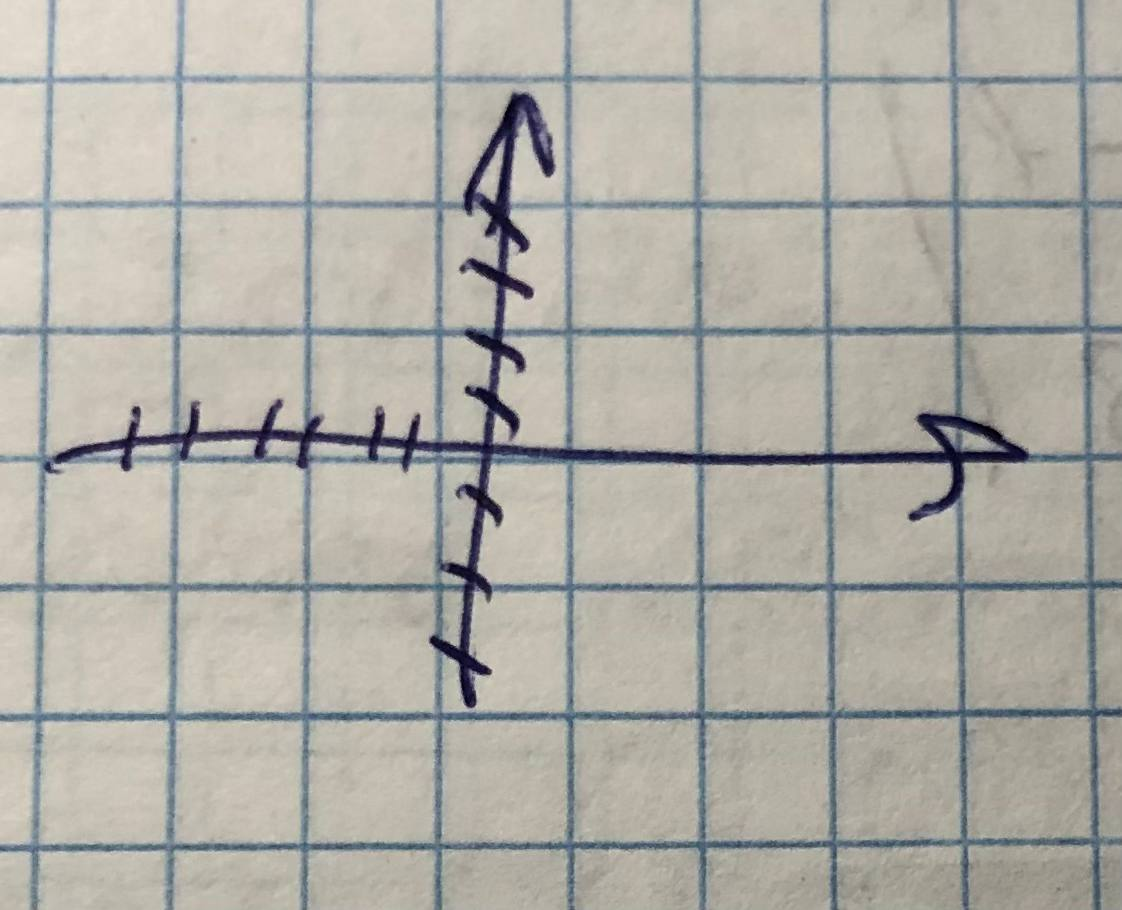
\includegraphics[width=3in,height=3in]{system_one_for_zerox_4.jpeg}
\end{center}

\item Пусть $y = 0$
\[
\begin{cases}
\frac{dx}{dt} = 9x \\
\frac{dy}{dt} = 5x
\end{cases}
\]
\begin{center}
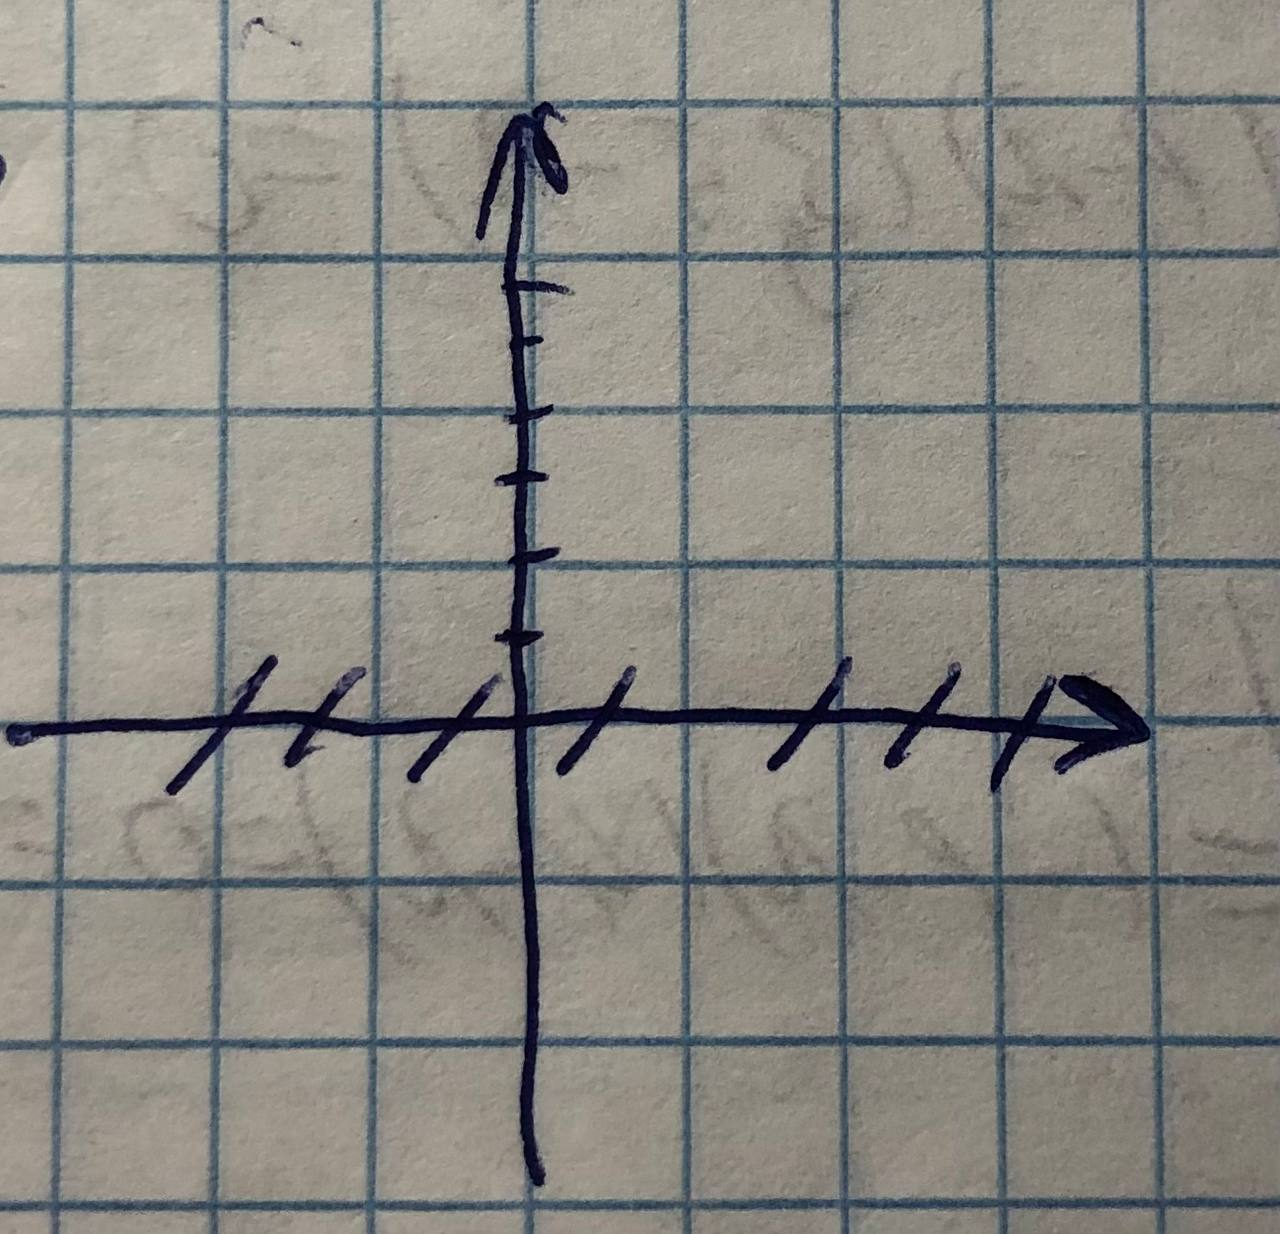
\includegraphics[width=3in,height=3in]{system_one_for_zeroy_4.jpeg}
\end{center}

\end{enumerate}

\begin{center}
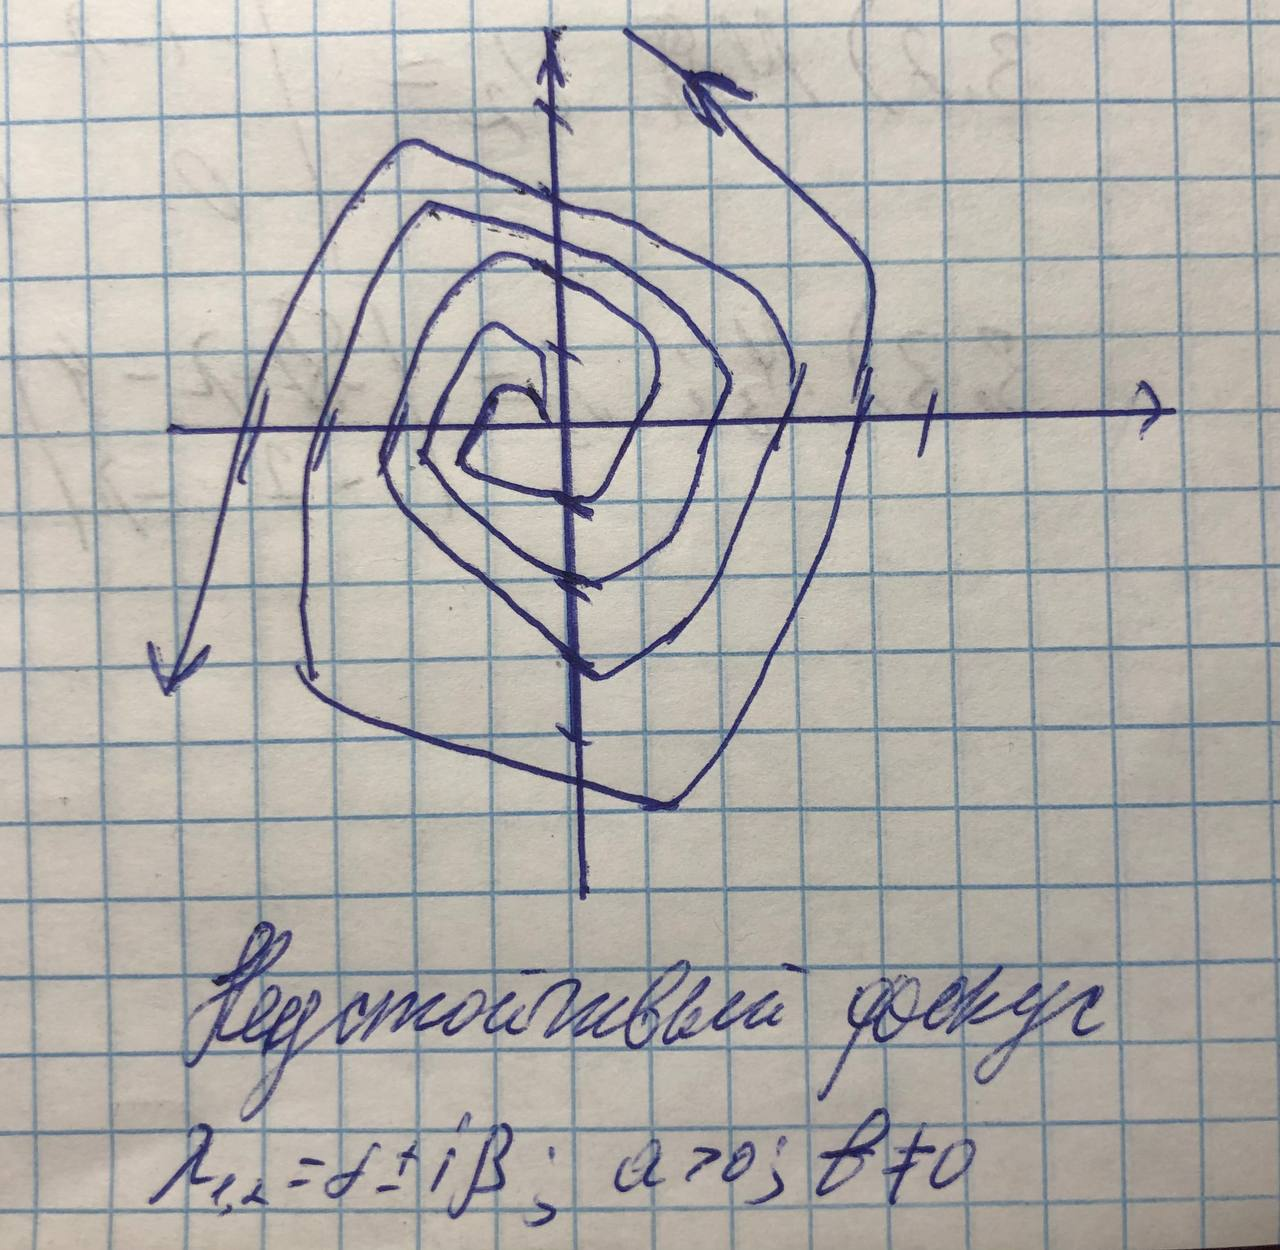
\includegraphics[width=3in,height=3in]{phase_trajectories.jpeg}
\end{center}

\subsection{Исследование динамической системы}

Мы рассматриваем динамическую систему с дифференциальными уравнениями:

\[
\begin{aligned}
\frac{{dx}}{{dt}} &= 2x+y^2-1 \\
\frac{{dy}}{{dt}} &= 6x-y^2+1
\end{aligned}
\]

\subsubsection{1.Особые точки}

Для нахождения особых точек решим систему уравнений:

\[
\begin{aligned}
2x+y^2-1 &= 0 \\
 6x-y^2+1 &= 0
\end{aligned}
\]

Из этой системы получаем три особые точки:

\begin{itemize}
  \item $M_1 = (0, 1)$
  \item $M_2 = (0, -1)$
\end{itemize}

\subsubsection{2.Анализ особых точек}

Для каждой особой точки найдем якобиан системы:


\[
J(x, y) =
\begin{bmatrix}
\frac{{\partial f}}{{\partial x}} & \frac{{\partial f}}{{\partial y}} \\
\frac{{\partial g}}{{\partial x}} & \frac{{\partial g}}{{\partial y}} \\
\end{bmatrix}
=
\begin{bmatrix}
2 & 2y \\
 6 & -2y\\
\end{bmatrix}
\]

Вычислим якобиан в каждой особой точке:


\begin{itemize}
  \item $M_1 = (0, 1)$:
  
  Якобиан $J(0, 1) = \begin{bmatrix} 2 & 2 \\ 6 & -2 \end{bmatrix}$
  
  Определитель: $\det(J(0, 1) - \lambda I) = \begin{vmatrix} 2-\lambda & 2 \\ 6 & -2-\lambda \end{vmatrix} = \lambda^2-16$
  
  Собственные значения: $\lambda_1 = 4$, $\lambda_2 = -4$

\begin{itemize}

\item Найдем собственный вектор для $\lamda_1 = 4$ :

\(
\begin{pmatrix}
-2 & 2 \\
6 & -6 \\
\end{pmatrix}
\begin{pmatrix}
\alpha \\
\beta \\
\end{pmatrix}
= 0
\)
  
Получается собственный вектор:
Вектор-столбец:
\(
\begin{pmatrix}
1 \\
1 \\
\end{pmatrix}
\)

\begin{center}
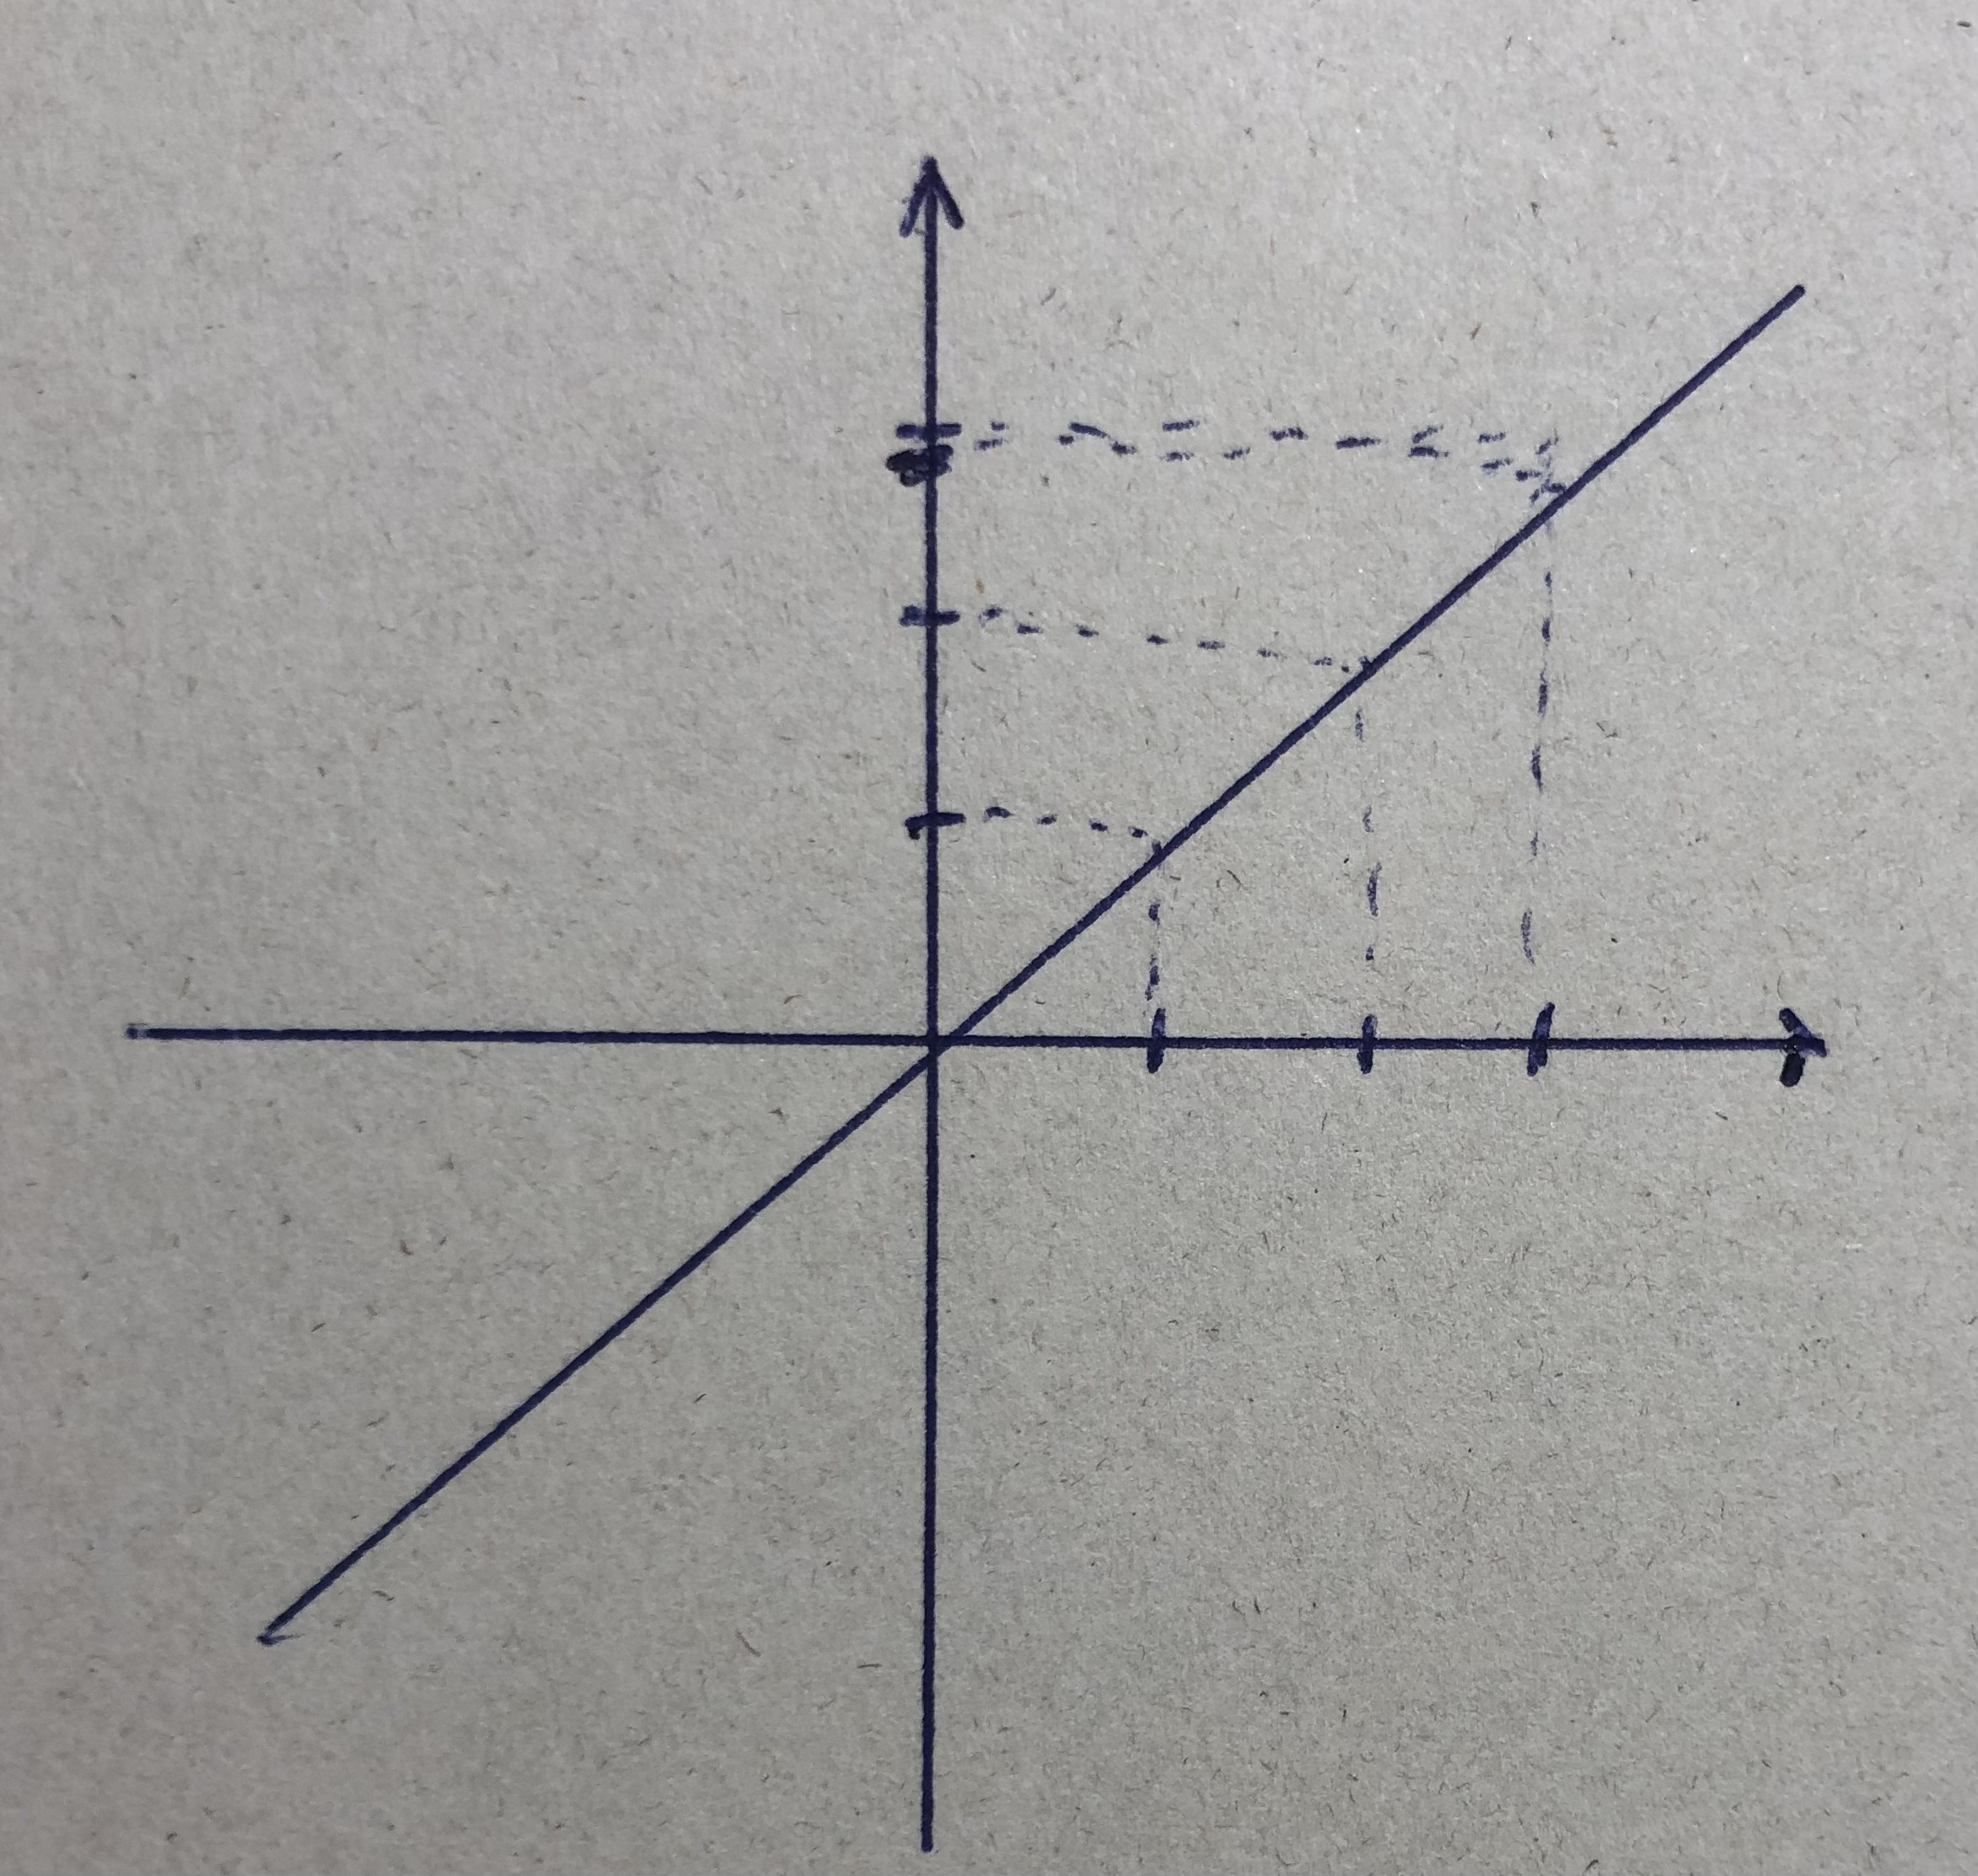
\includegraphics[width=3in,height=3in]{sobstveni_vector_5_1.jpeg}
\end{center}

\item Найдем собственный вектор для $\lamda_2 = -4$ :

\(
\begin{pmatrix}
6 & 2 \\
6 & 2 \\
\end{pmatrix}
\begin{pmatrix}
\alpha \\
\beta \\
\end{pmatrix}
= 0
\)
  
Получается собственный вектор:
Вектор-столбец:
\(
\begin{pmatrix}
-1 \\
3 \\
\end{pmatrix}
\)

\begin{center}
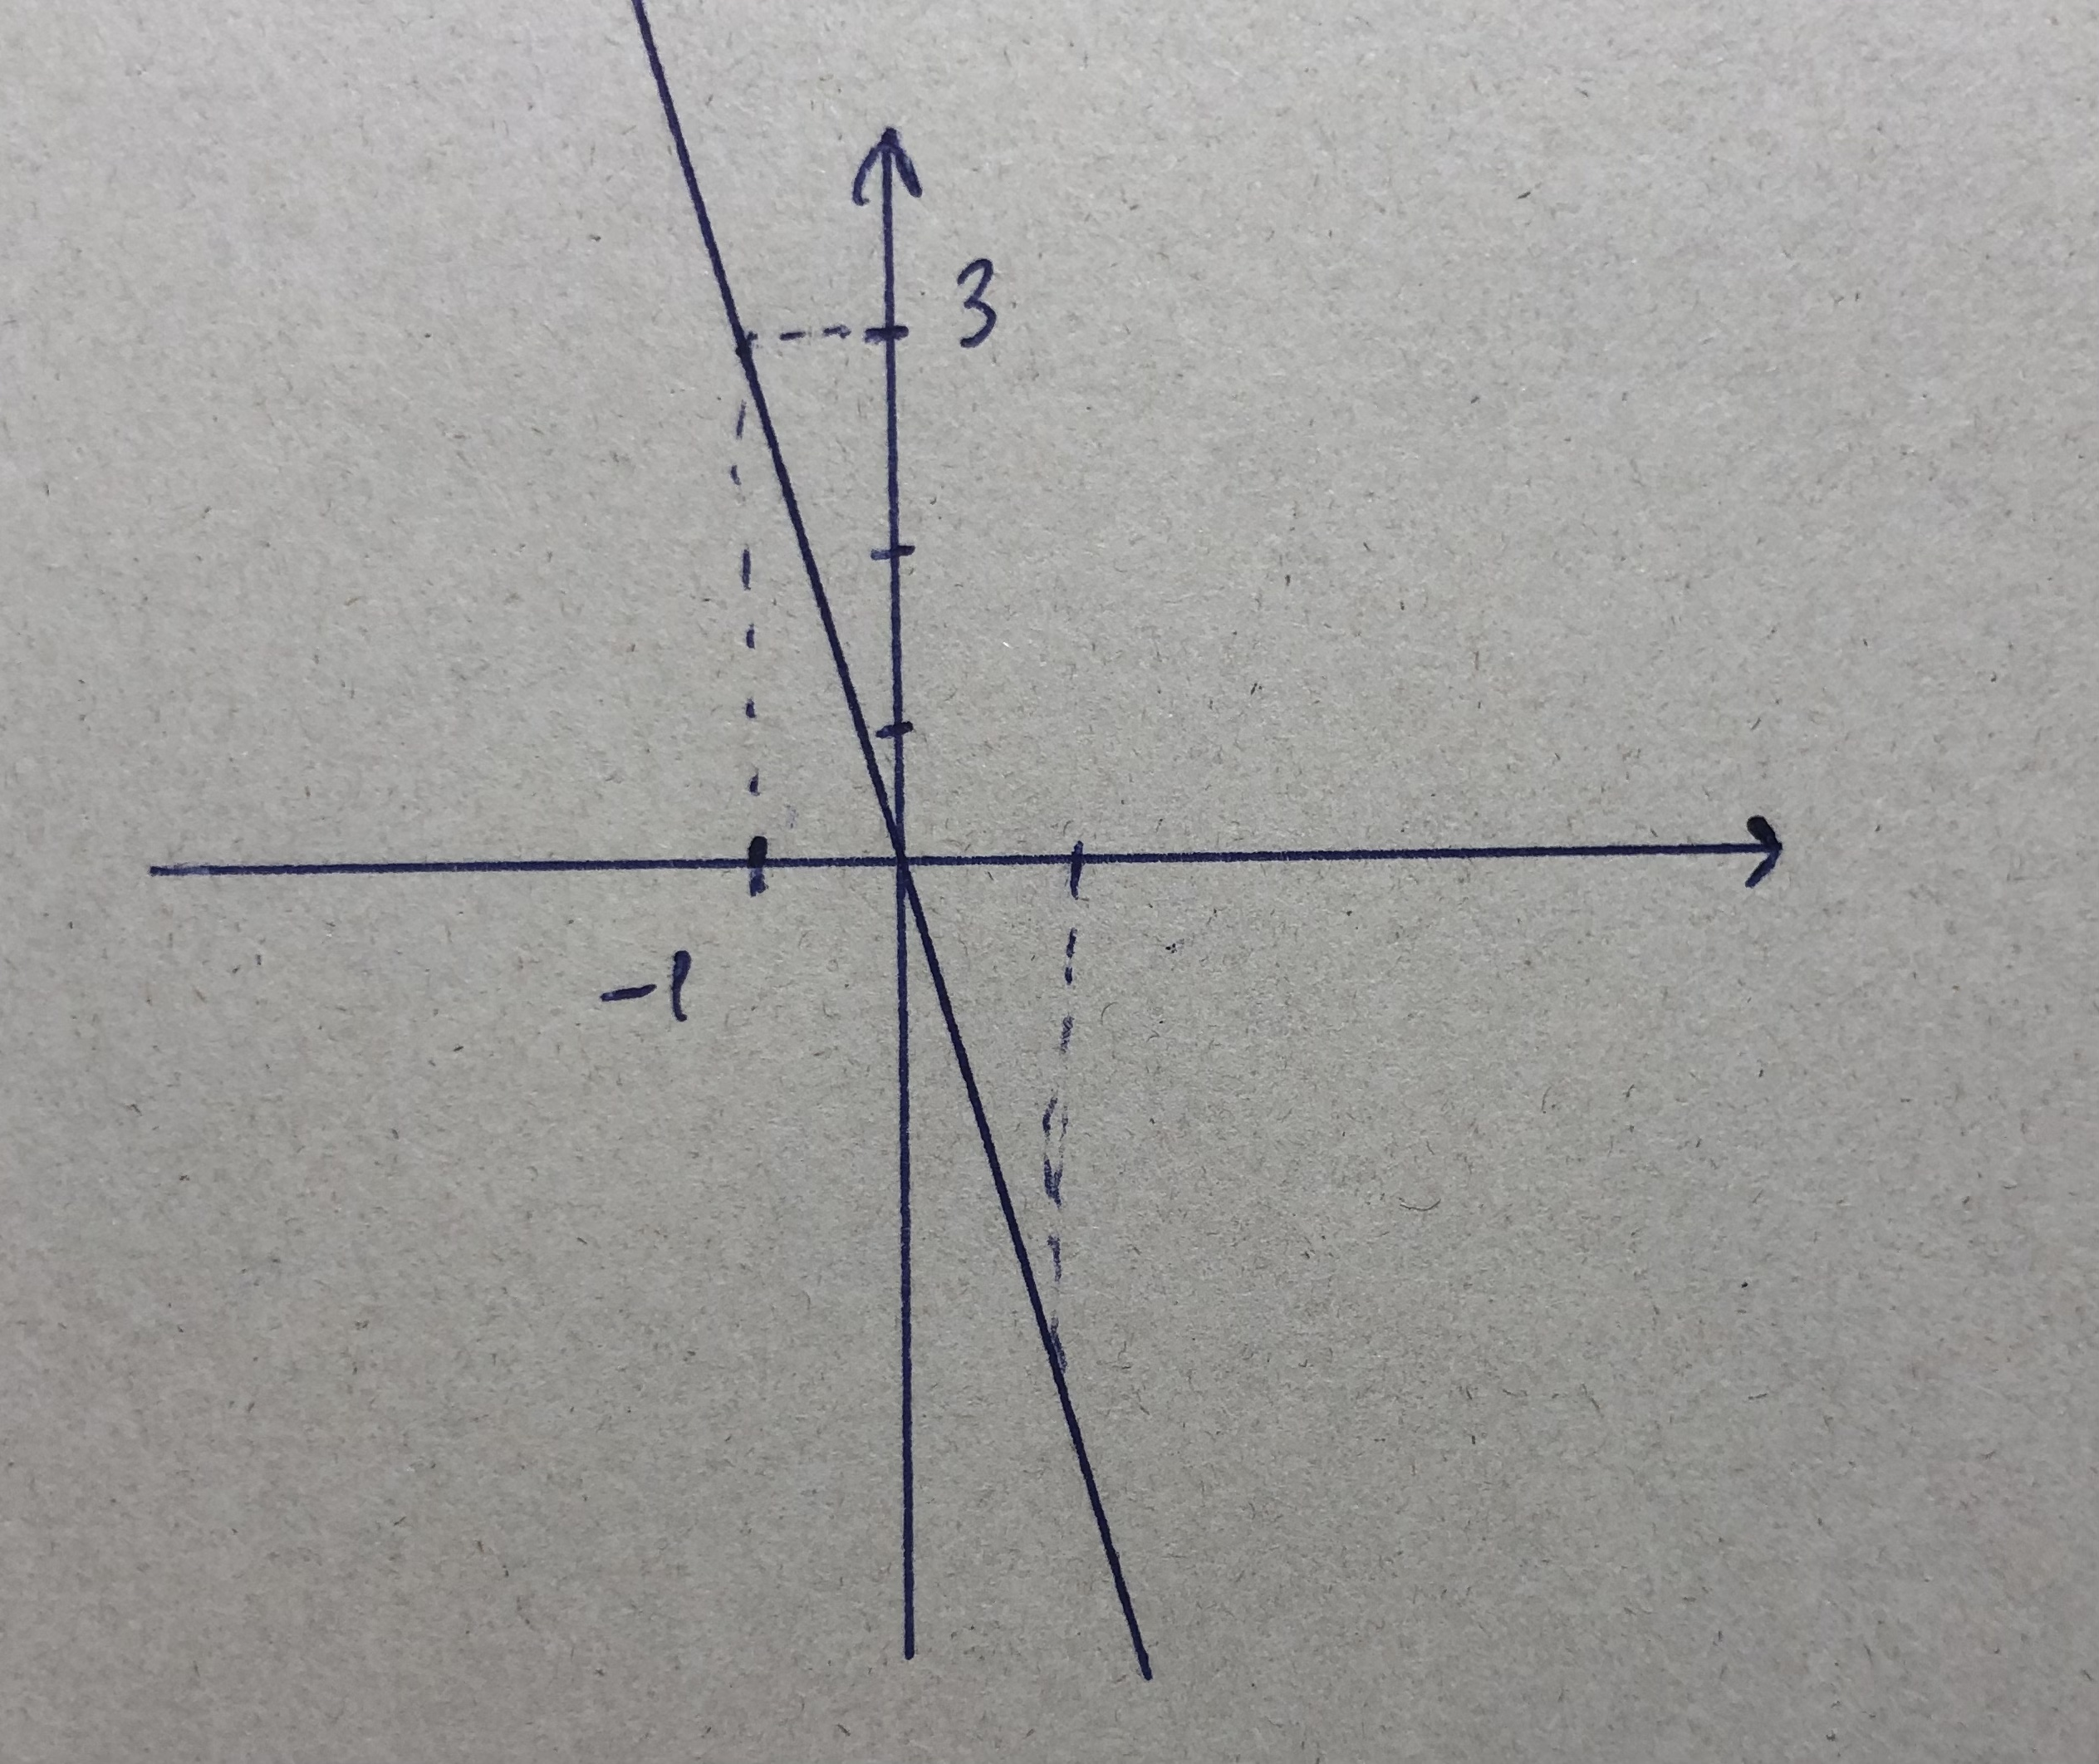
\includegraphics[width=3in,height=3in]{sobstveni_vector_5_2.jpeg}
\end{center}

Сделаем замену :

\[
\left\{
\begin{aligned}
u &= x - 0 \\
v &= y - 1
\end{aligned}
\right.
\Rightarrow
\left\{
\begin{aligned}
x &= u \\
y &= v + 1
\end{aligned}
\right.
\]

Подставим в изначальную систему:

\[
\begin{aligned}
\dot{u} &= v^2 + 2u + 2v \\
\dot{v} &= -v^2 + 6u - 2v \\
\end{aligned}
\]

Оставим только линейную часть:

\[
\begin{aligned}
\dot{u} &= 2u + 2v \\
\dot{v} &= 6u - 2v \\
\end{aligned}
\]

\begin{itemize}
\item Пусть $u = 0$
        \[
\begin{cases}
\dot{u} = 2v \\
\dot{v} = -2v
\end{cases}
\]
\begin{center}
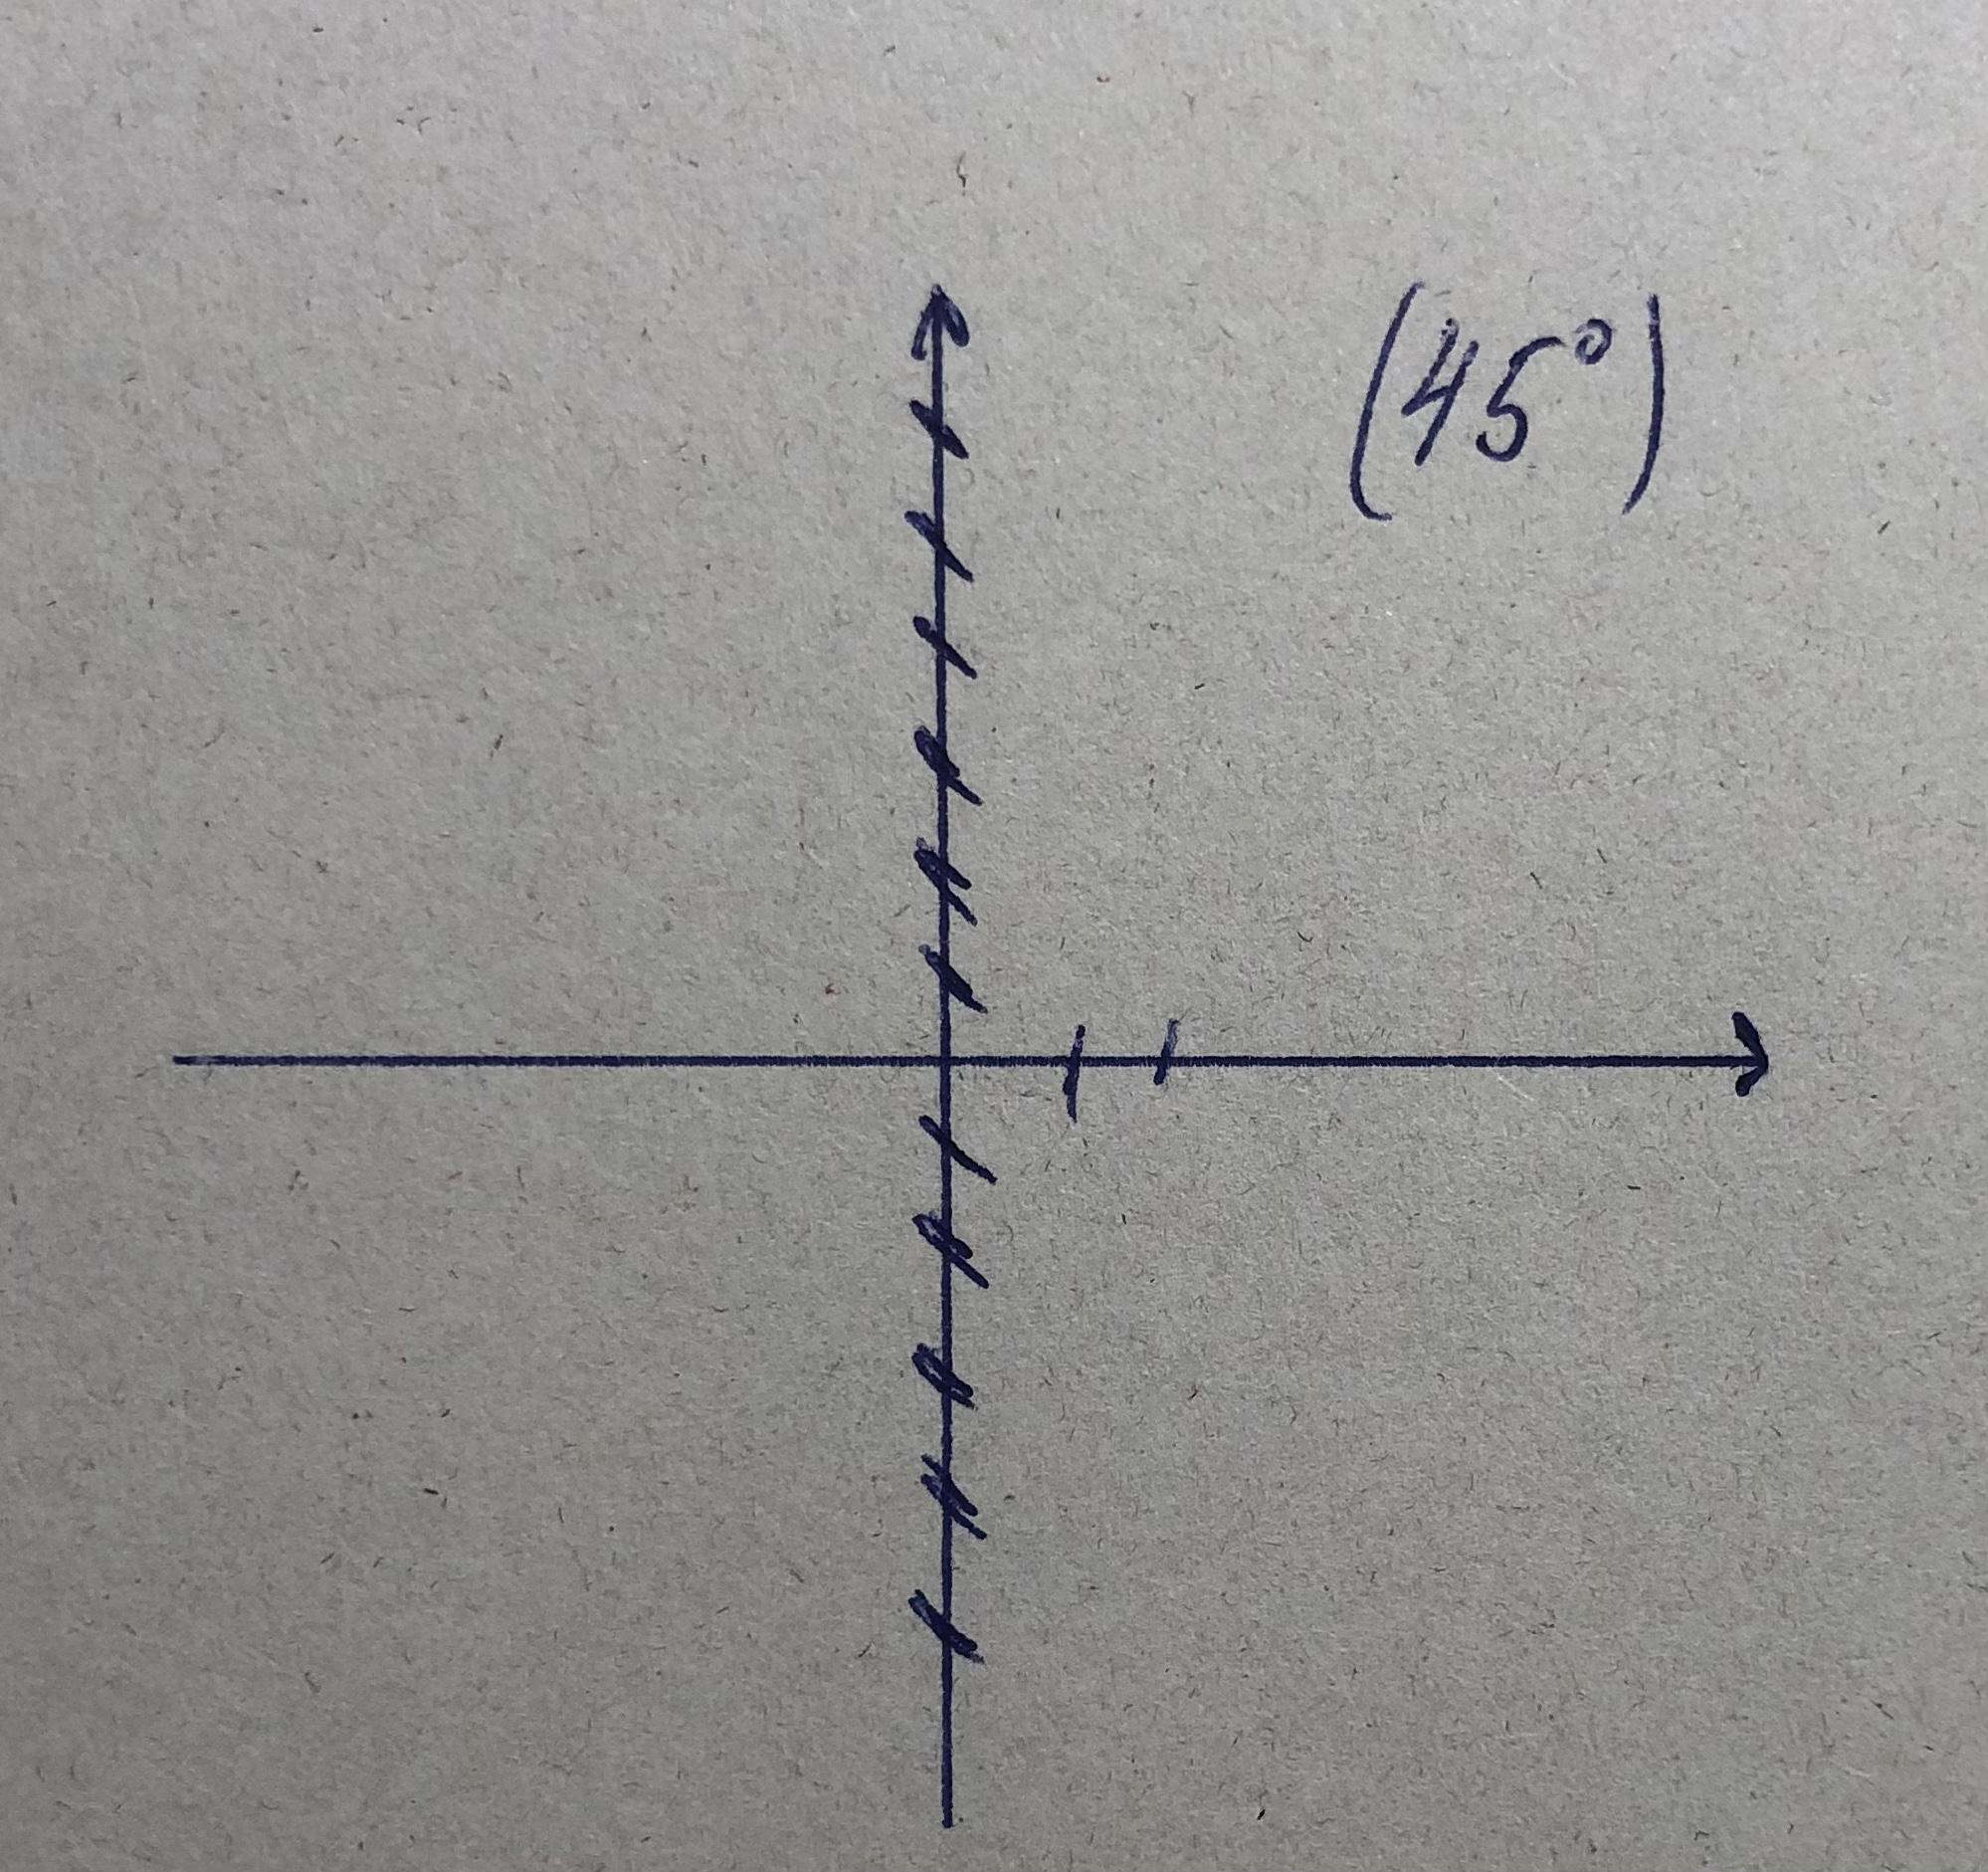
\includegraphics[width=3in,height=3in]{system_one_for_zerou_5.jpeg}
\end{center}

\item Пусть $v = 0$
        \[
\begin{cases}
\dot{u} = 2u \\
\dot{v} = 6u
\end{cases}
\]
\begin{center}
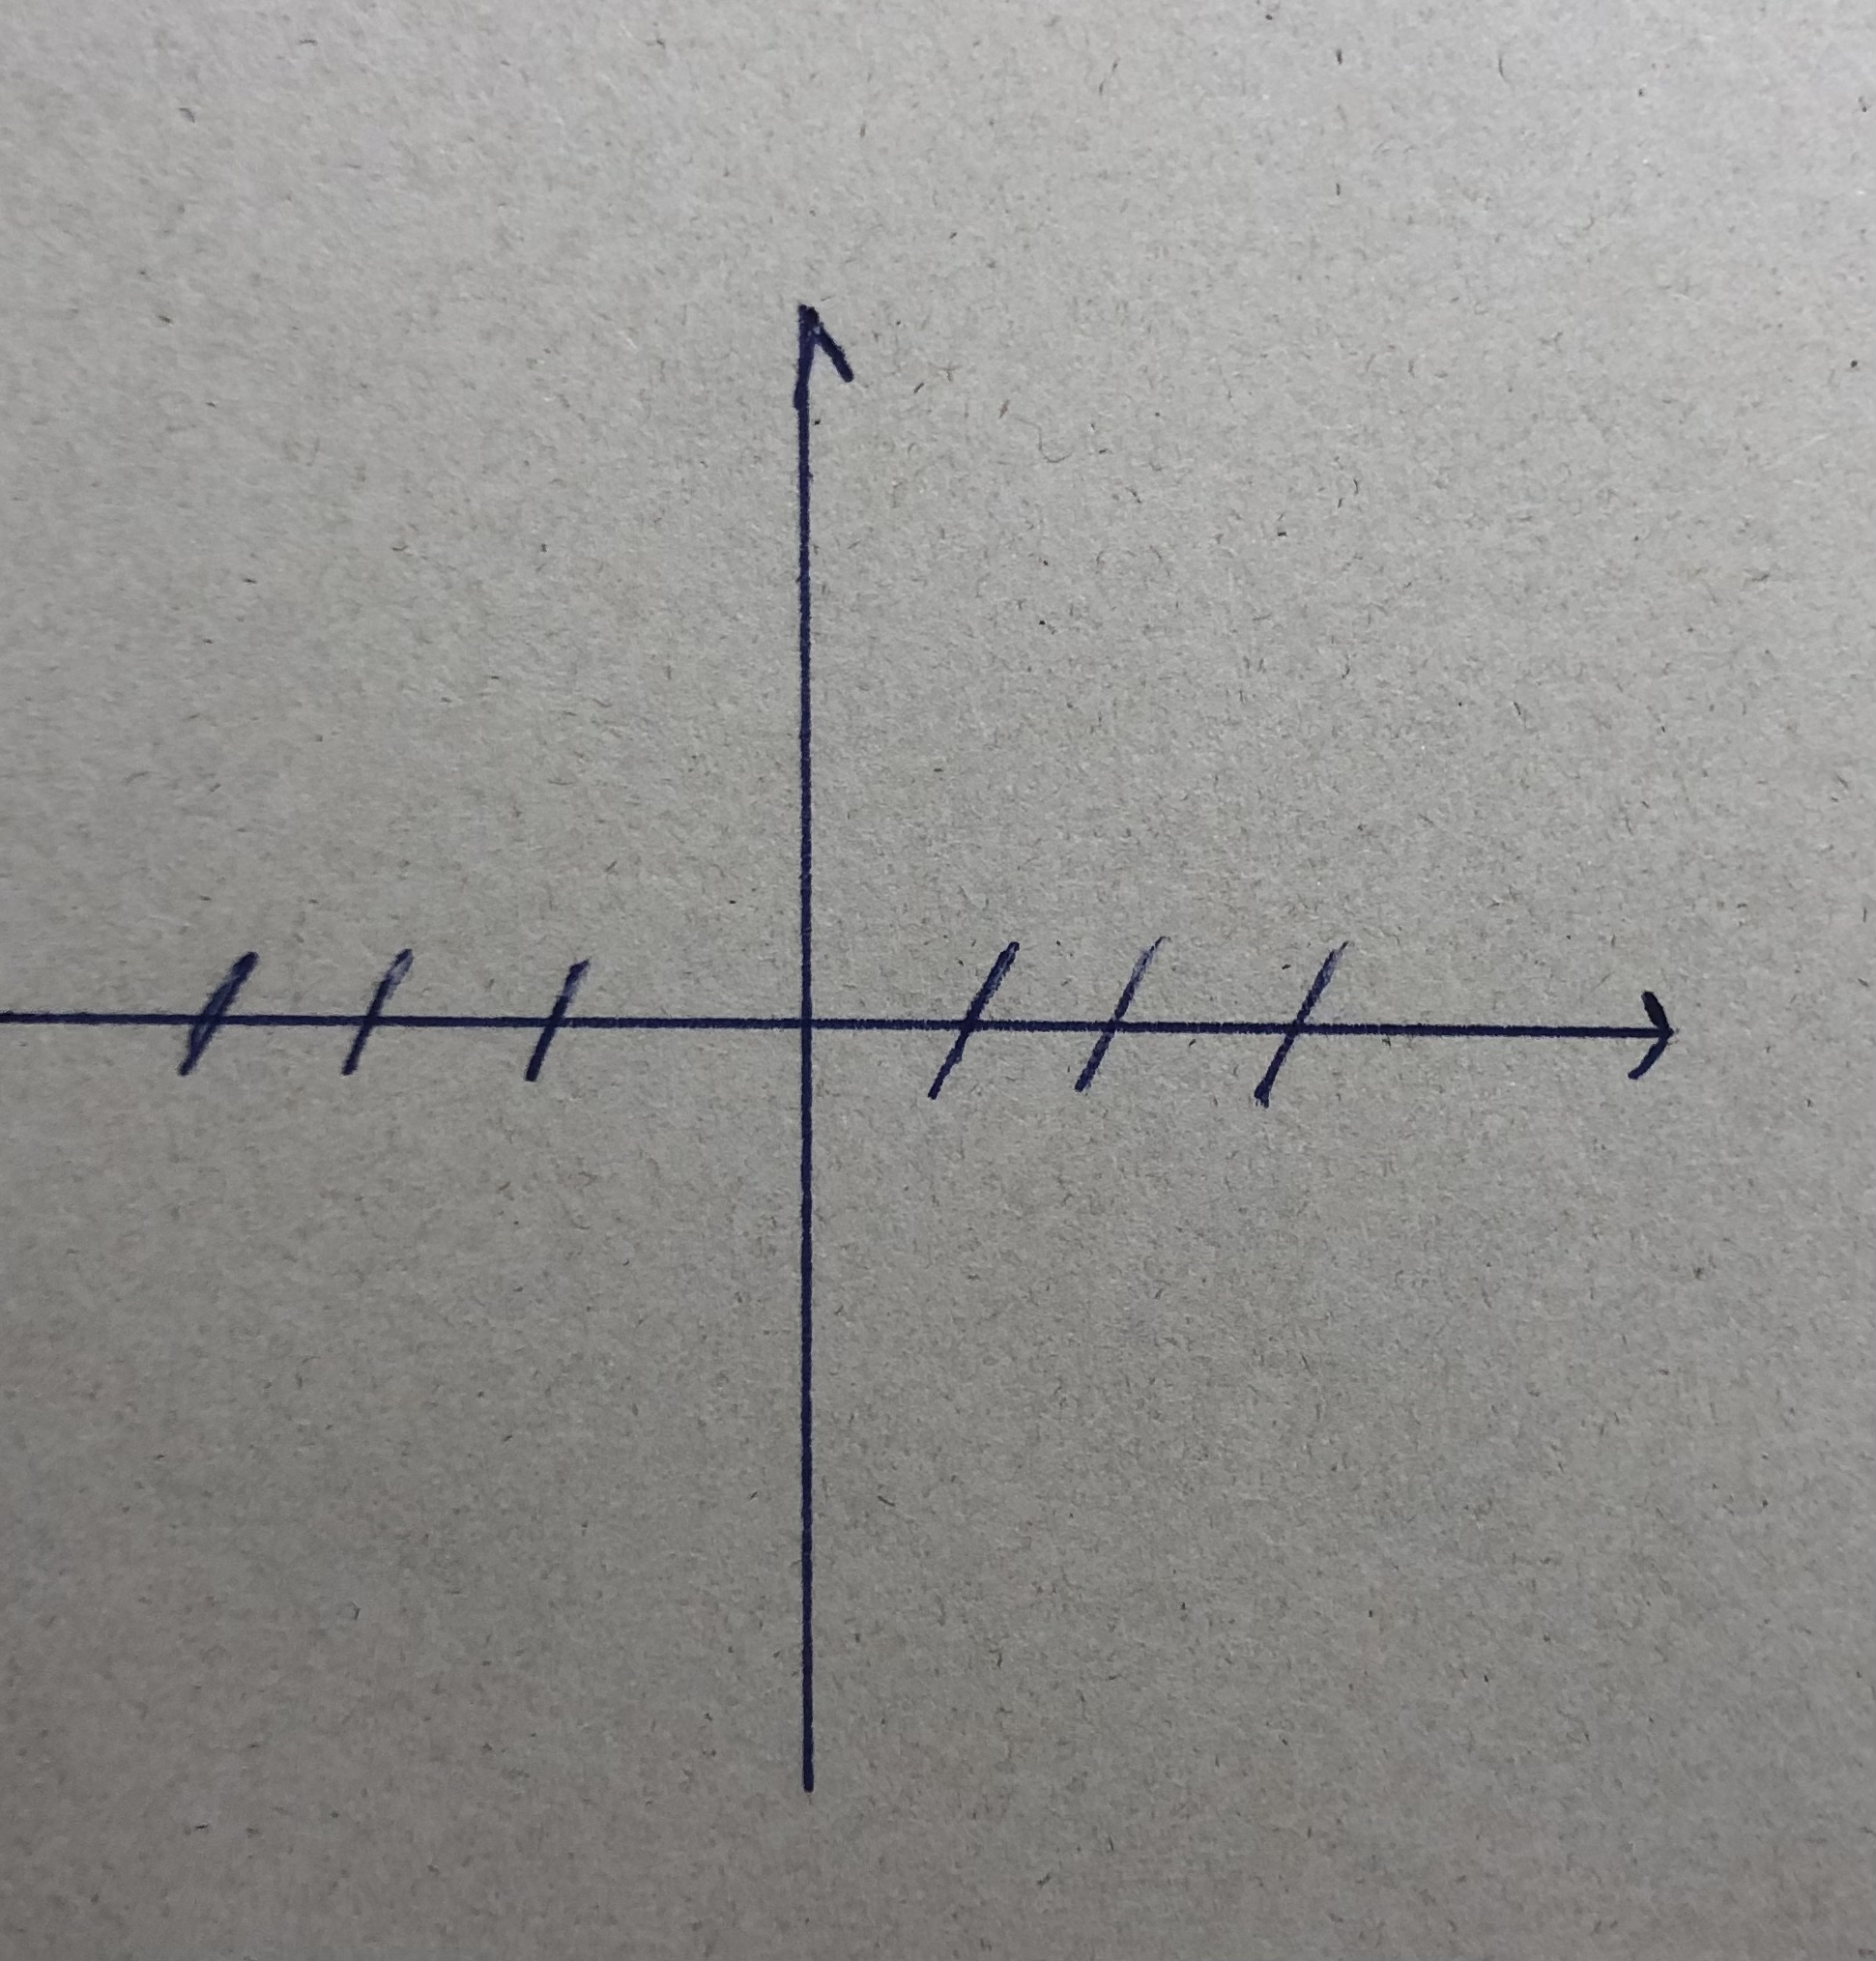
\includegraphics[width=3in,height=3in]{system_one_for_zerov_5.jpeg}
\end{center}

\item Пусть $\dot{v} = 0 \Rightarrow 3u=v$
\begin{center}
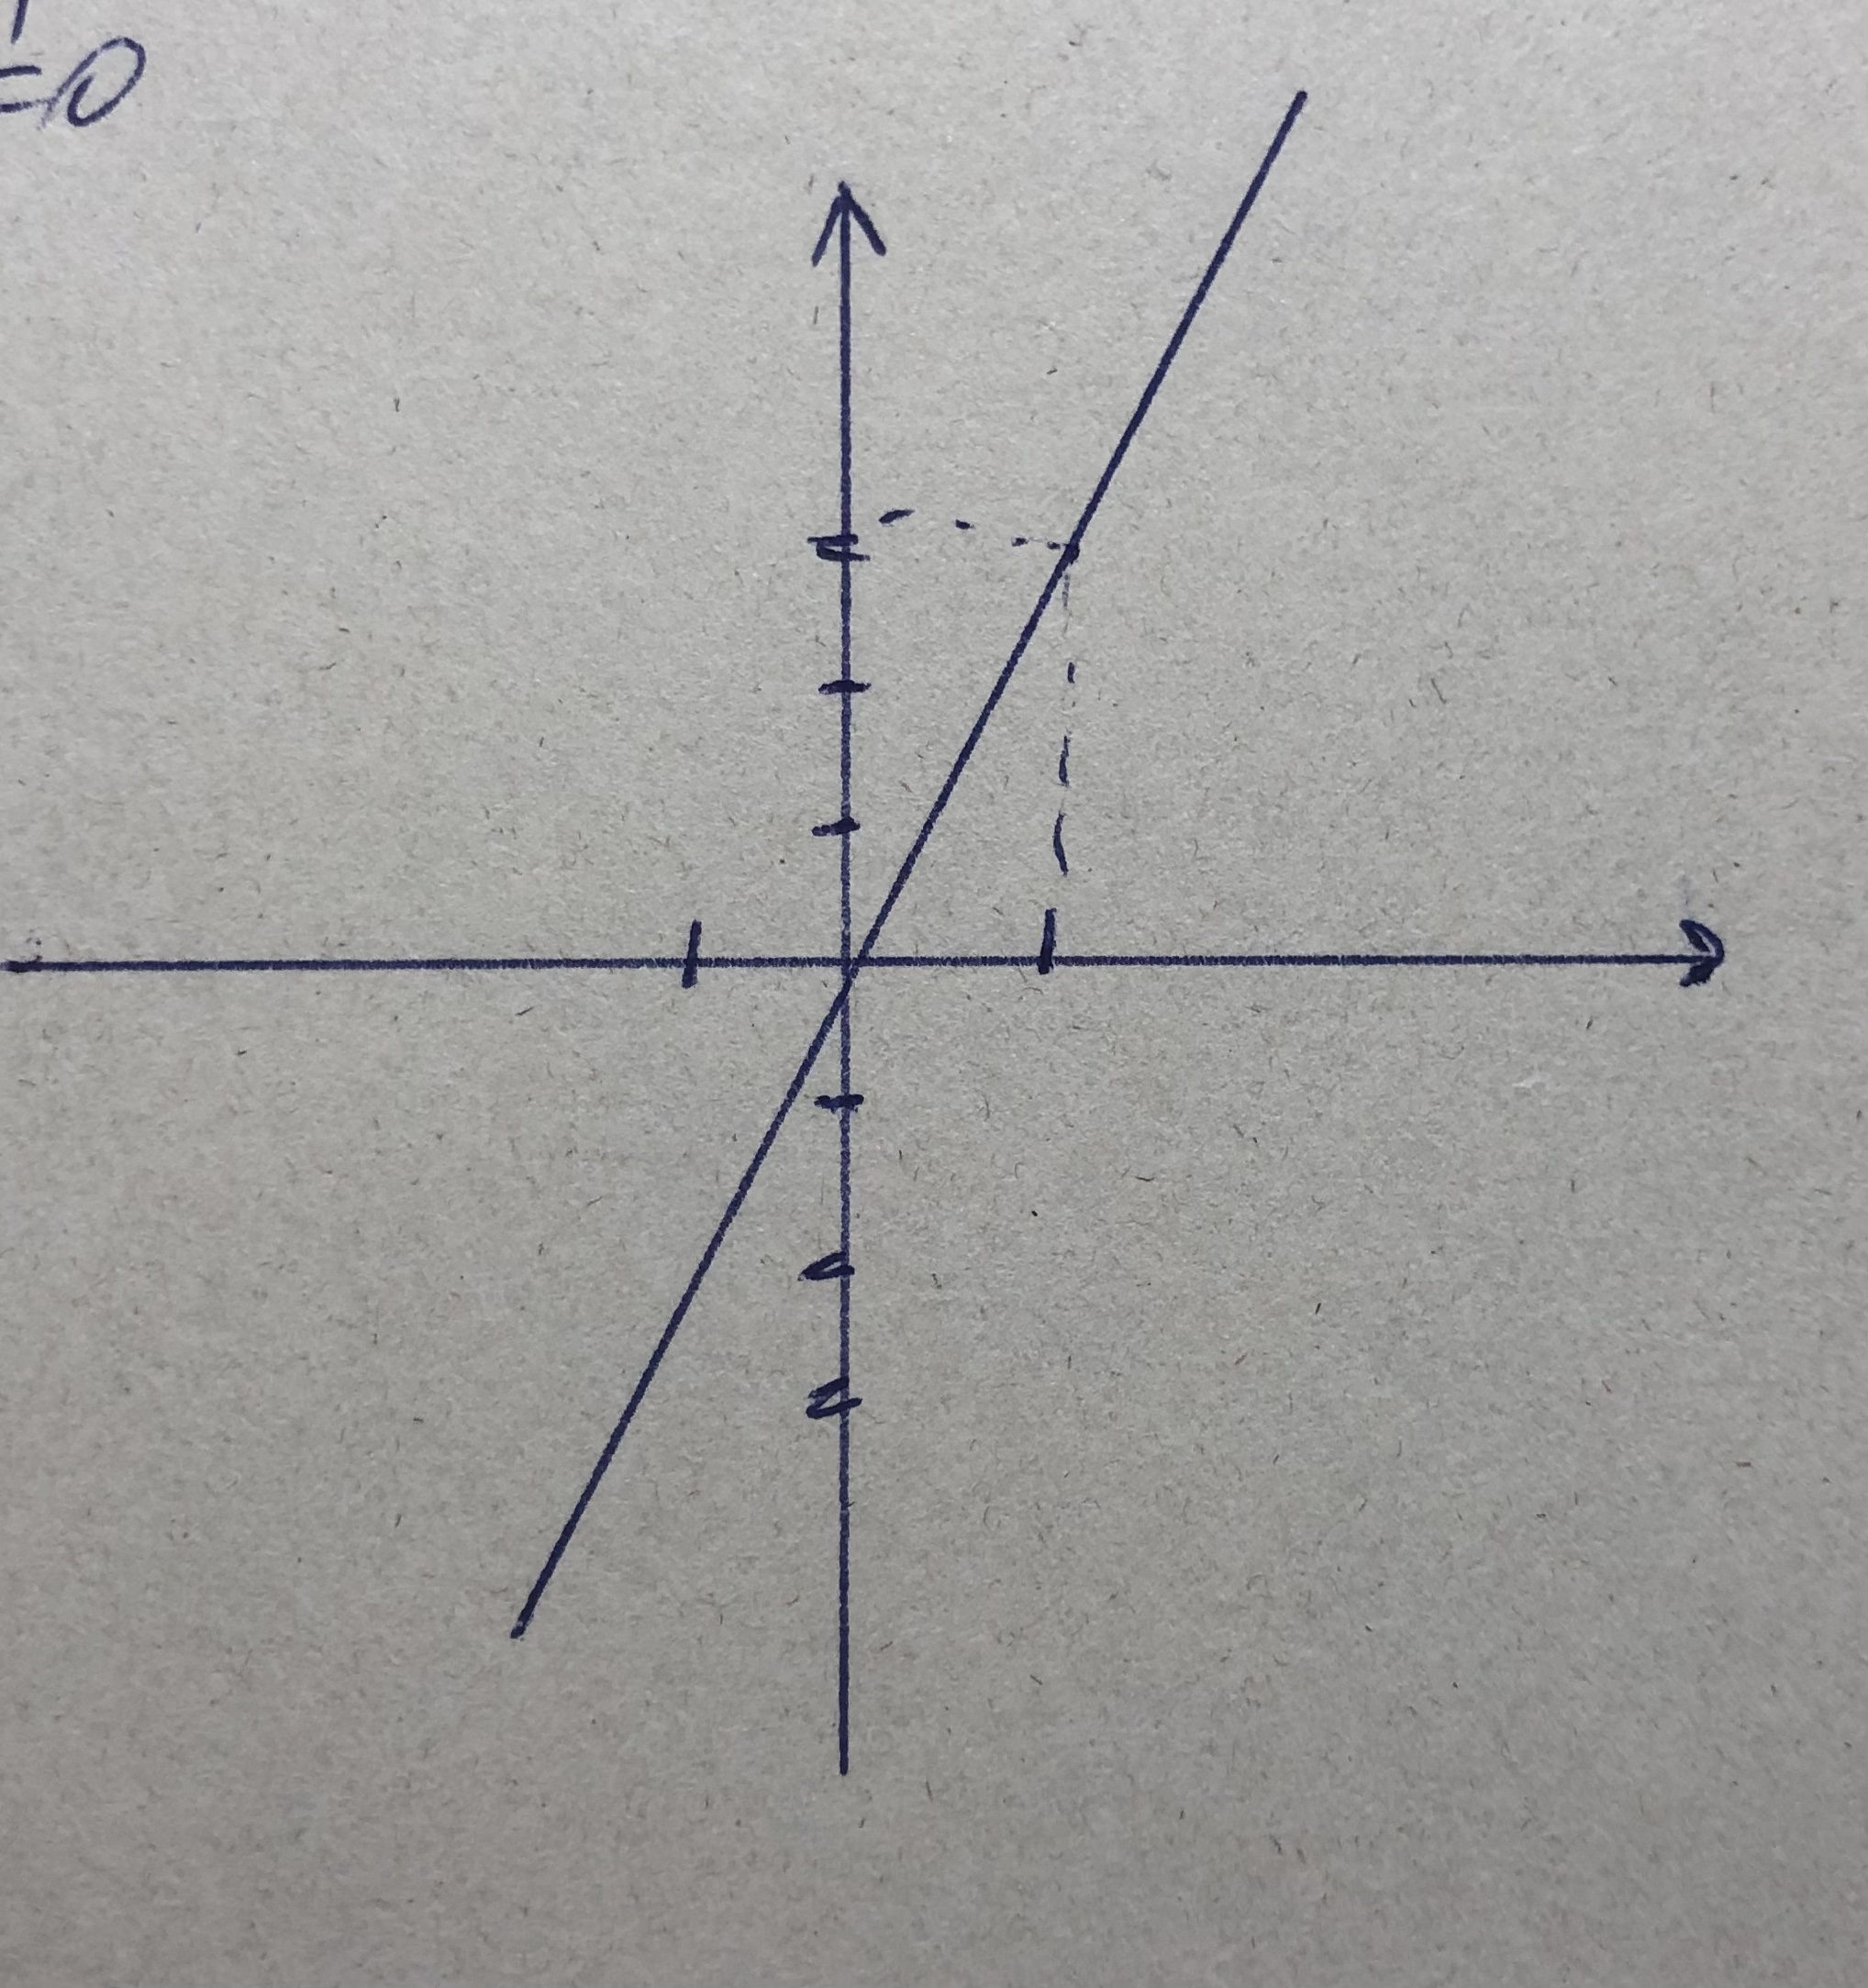
\includegraphics[width=3in,height=3in]{system_one_for_zerov_shtrih_5.jpeg}
\end{center}

\end{itemize}

\end{itemize}

  \item $M_2 = (0, -1)$:
  
  Якобиан $J(0, -1) = \begin{bmatrix} 2 & -2 \\ 6 & 2 \end{bmatrix}$
  
  Определитель:\[
\det(J(0, -1) - \lambda I) = \begin{vmatrix} 2-\lambda & -2 \\ 6 & 2-\lambda \end{vmatrix} = (2-\lambda)^2 + 12.
\]
  
  Собственные значения: $\lambda_3 = 2+\sqrt{3i}$, $\lambda_4 = 2-\sqrt{3i}$

  Сделаем замену :

\[
\left\{
\begin{aligned}
u &= x - 0 \\
v &= y + 1
\end{aligned}
\right.
\Rightarrow
\left\{
\begin{aligned}
x &= u \\
y &= v - 1
\end{aligned}
\right.
\]

Подставим в изначальную систему:

\[
\begin{aligned}
\dot{u} &= v^2 + 2u - 2v \\
\dot{v} &= -v^2 + 6u + 2v \\
\end{aligned}
\]

Оставим только линейную часть:

\[
\begin{aligned}
\dot{u} &= 2u - 2v \\
\dot{v} &= 6u + 2v \\
\end{aligned}
\]

\begin{itemize}
\item Пусть $u = 0$
        \[
\begin{cases}
\dot{u} = -2v \\
\dot{v} = 2v
\end{cases}
\]
\begin{center}
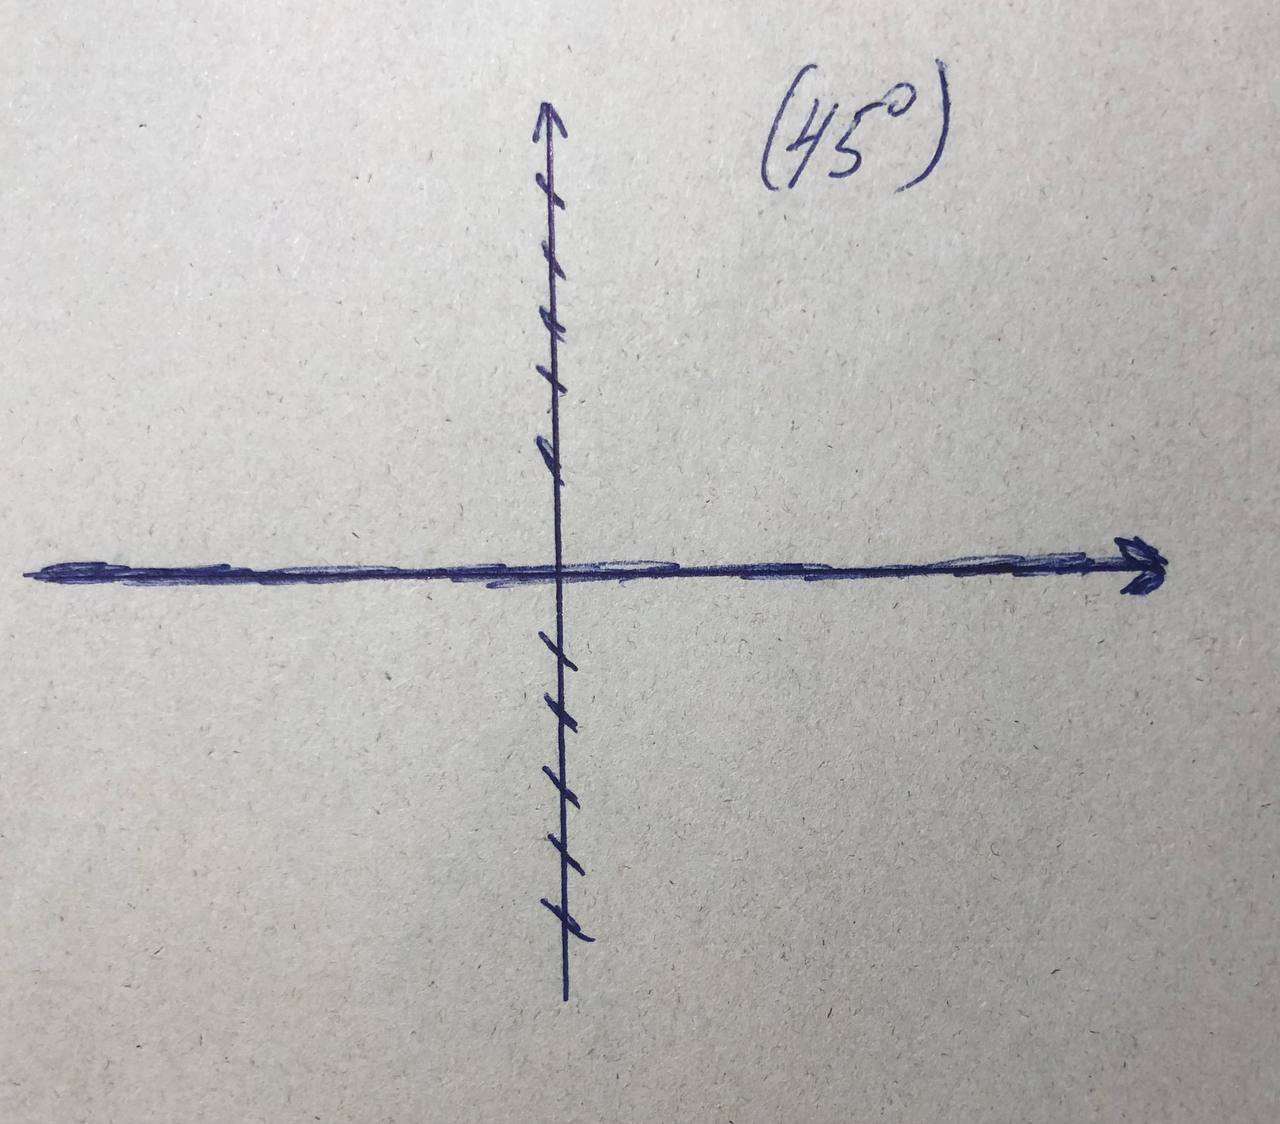
\includegraphics[width=3in,height=3in]{system_two_for_zerou_5.jpeg}
\end{center}

\item Пусть $v = 0$
        \[
\begin{cases}
\dot{u} = 2u \\
\dot{v} = 6u
\end{cases}
\]
\begin{center}
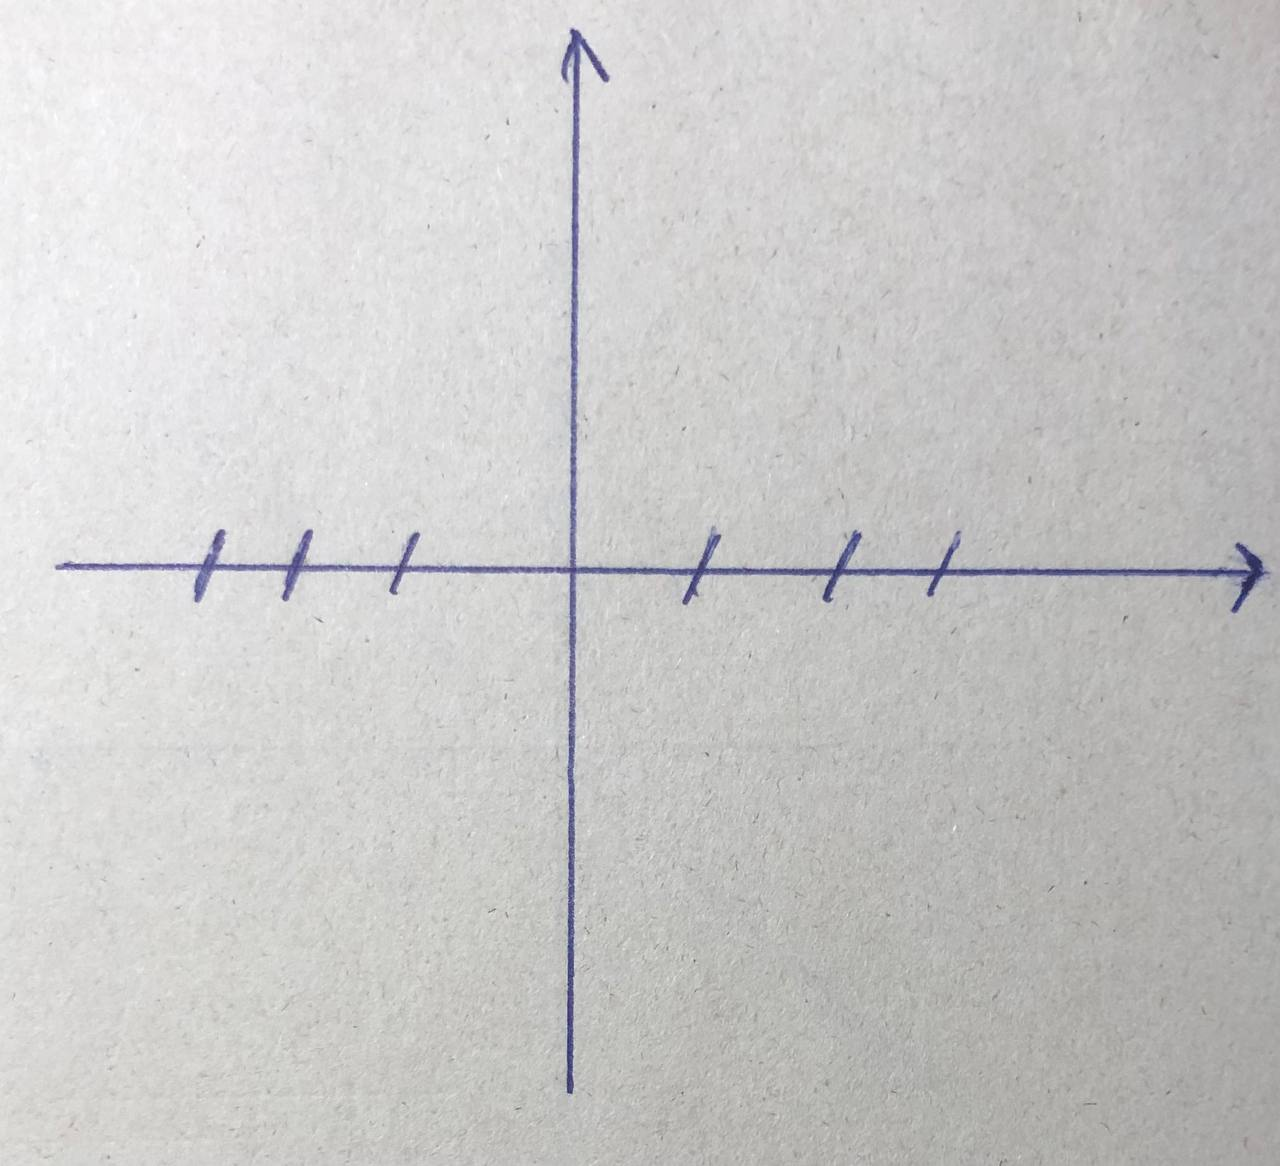
\includegraphics[width=3in,height=3in]{system_two_for_zerov_5.jpeg}
\end{center}

\end{itemize}
  
\end{itemize}

\clearpage

\subsubsection{3.Фазовый портрет}

Построим фазовый портрет для каждой особой точки и общий фазовый портрет, объединяющий локальные особые точки.

\begin{center}
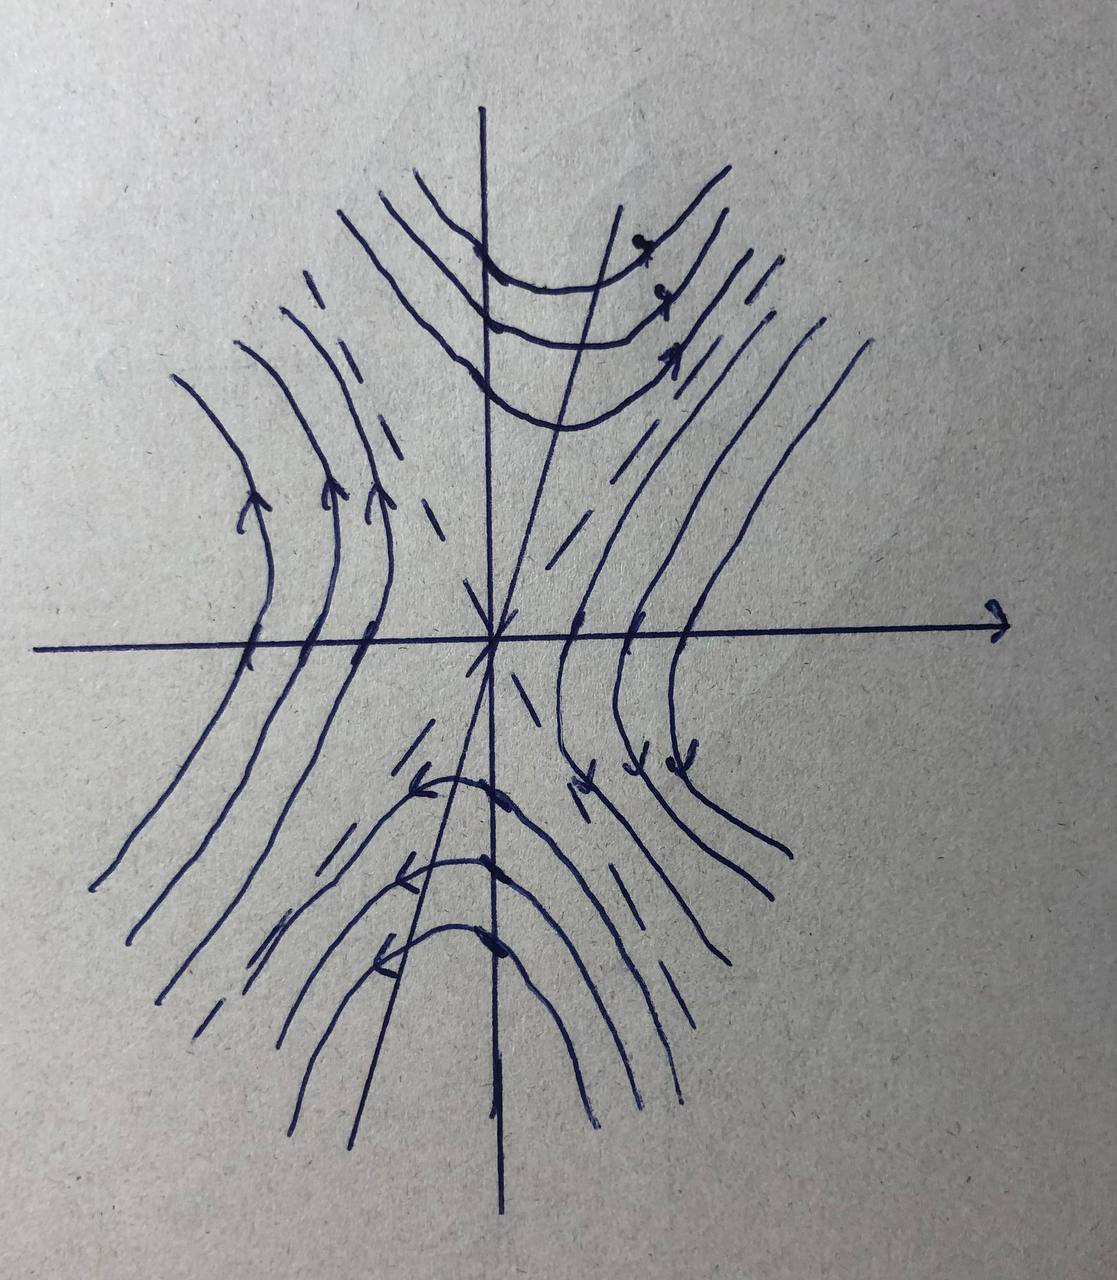
\includegraphics[width=0.6\textwidth]{phase_portret_sedlo5.png}
\captionof{figure}{Фазовый портрет в окрестности $M_1$ "седло"}
\end{center}

\begin{center}
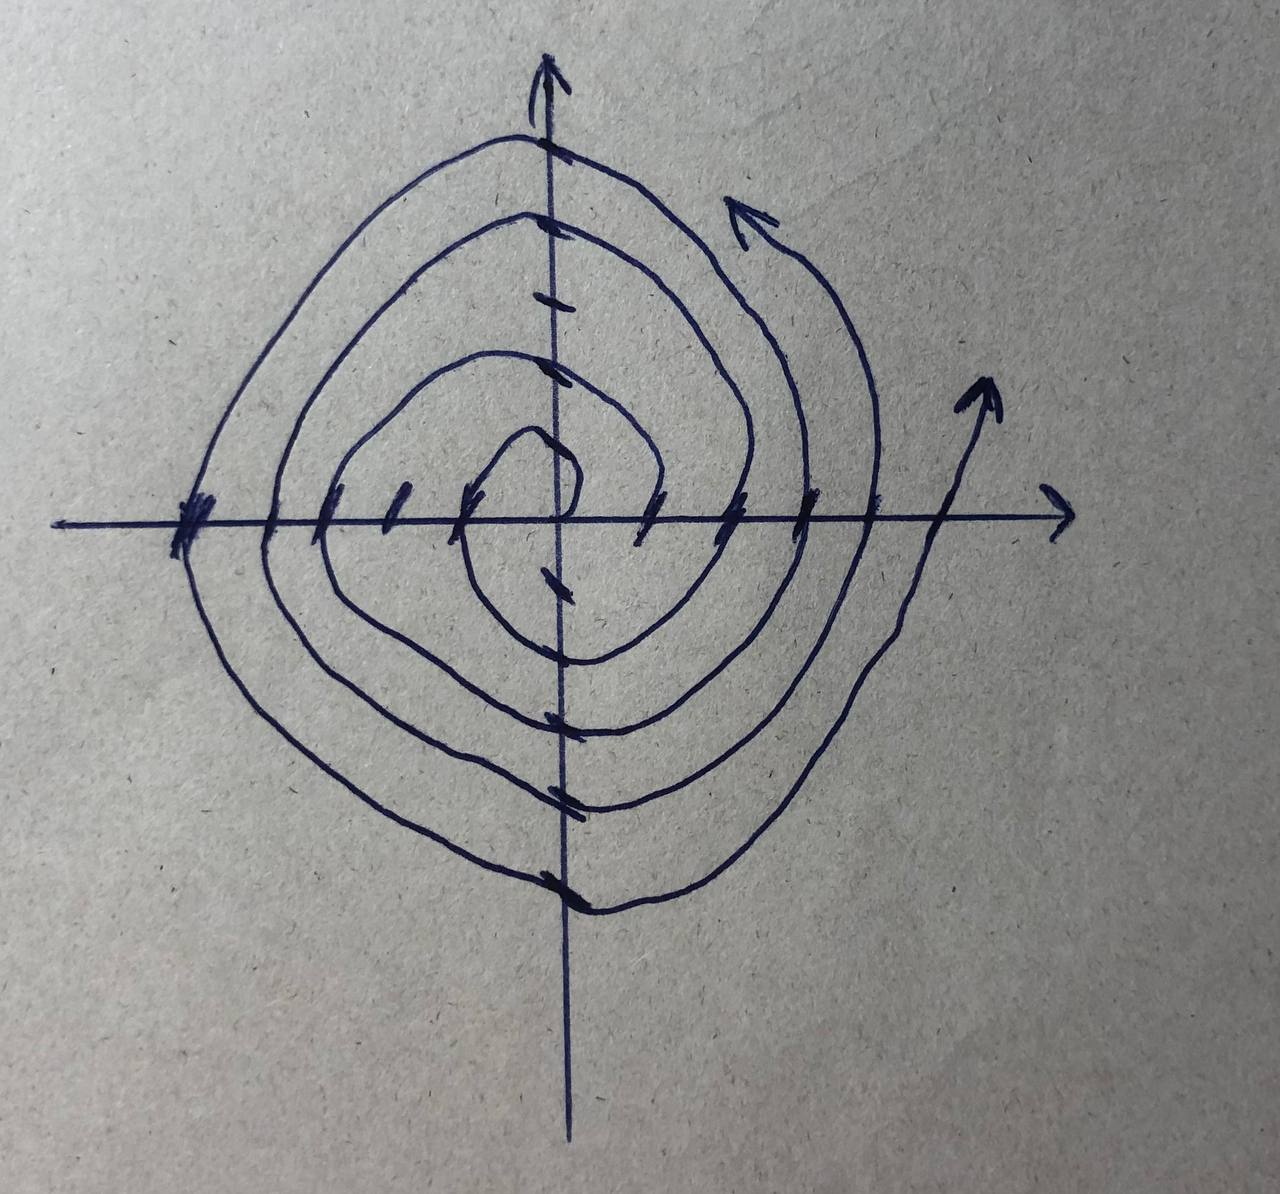
\includegraphics[width=0.6\textwidth]{phase_portret_ne_ust_uzel5.png}
\captionof{figure}{Фазовый портрет в окрестности $M_2$ "неустойчивый узел"}
\end{center}

\begin{center}
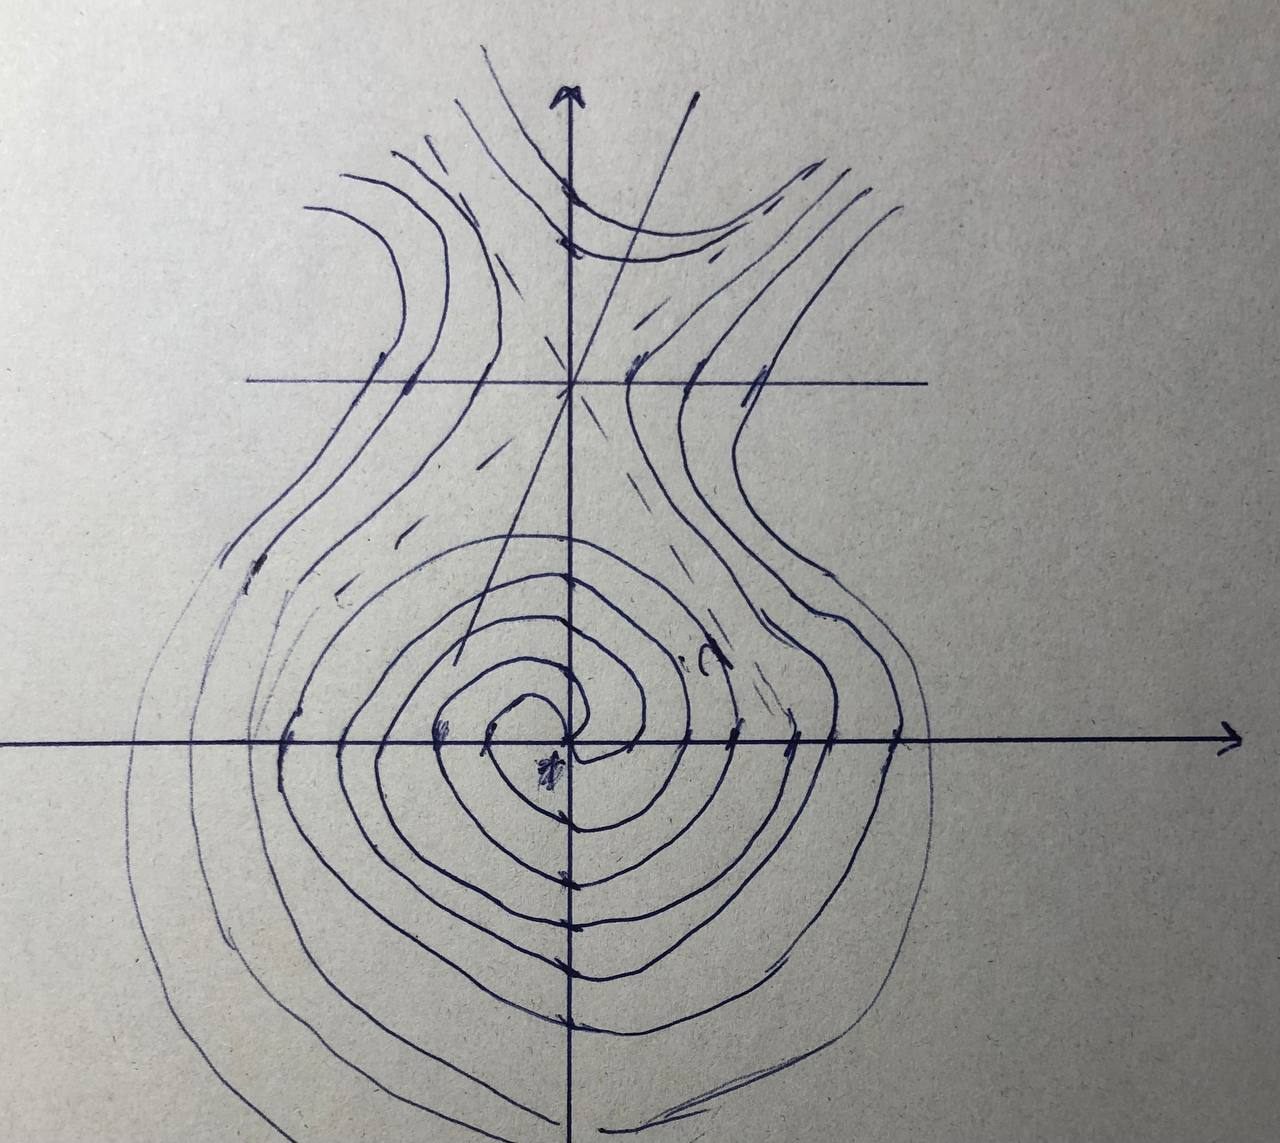
\includegraphics[width=0.6\textwidth]{phase_portret_obshi5.png}
\captionof{figure}{Общий фазовый портрет, объединяющий $M_1$ и $M_2$}
\end{center}

\end{document}
